
%%%%%%%%%%%%%%%%%%%%%%% List of tables and figures %%%%%%%%%%%%%%%%%%%%%
\renewcommand{\thesection}{}
\numberwithin{equation}{section}
\section*{Appendices}
\addcontentsline{toc}{section}{Appendices}
\setstretch{1.1}
\listoffigures
\listoftables
\restoregeometry
\setcounter{figure}{0}
\renewcommand{\thefigure}{A\arabic{figure}}
\setcounter{table}{0}
\renewcommand{\thetable}{B\arabic{table}}
\setstretch{1.5}
\clearpage

%%%%%%%%%%%%%%%%%%%%%%% Appendix A (Figures) %%%%%%%%%%%%%%%%%%%%% 
\renewcommand\thesubsection{A}
\subsection{Figures}

\begin{figure}[ht]
	\centering
	\caption[Comparison of CRSP returns]{Plots of CRSP reported holding period returns against daily close/open retuns}
	
	\begin{tabular}{cccc}
		\subfloat[Year 1997]{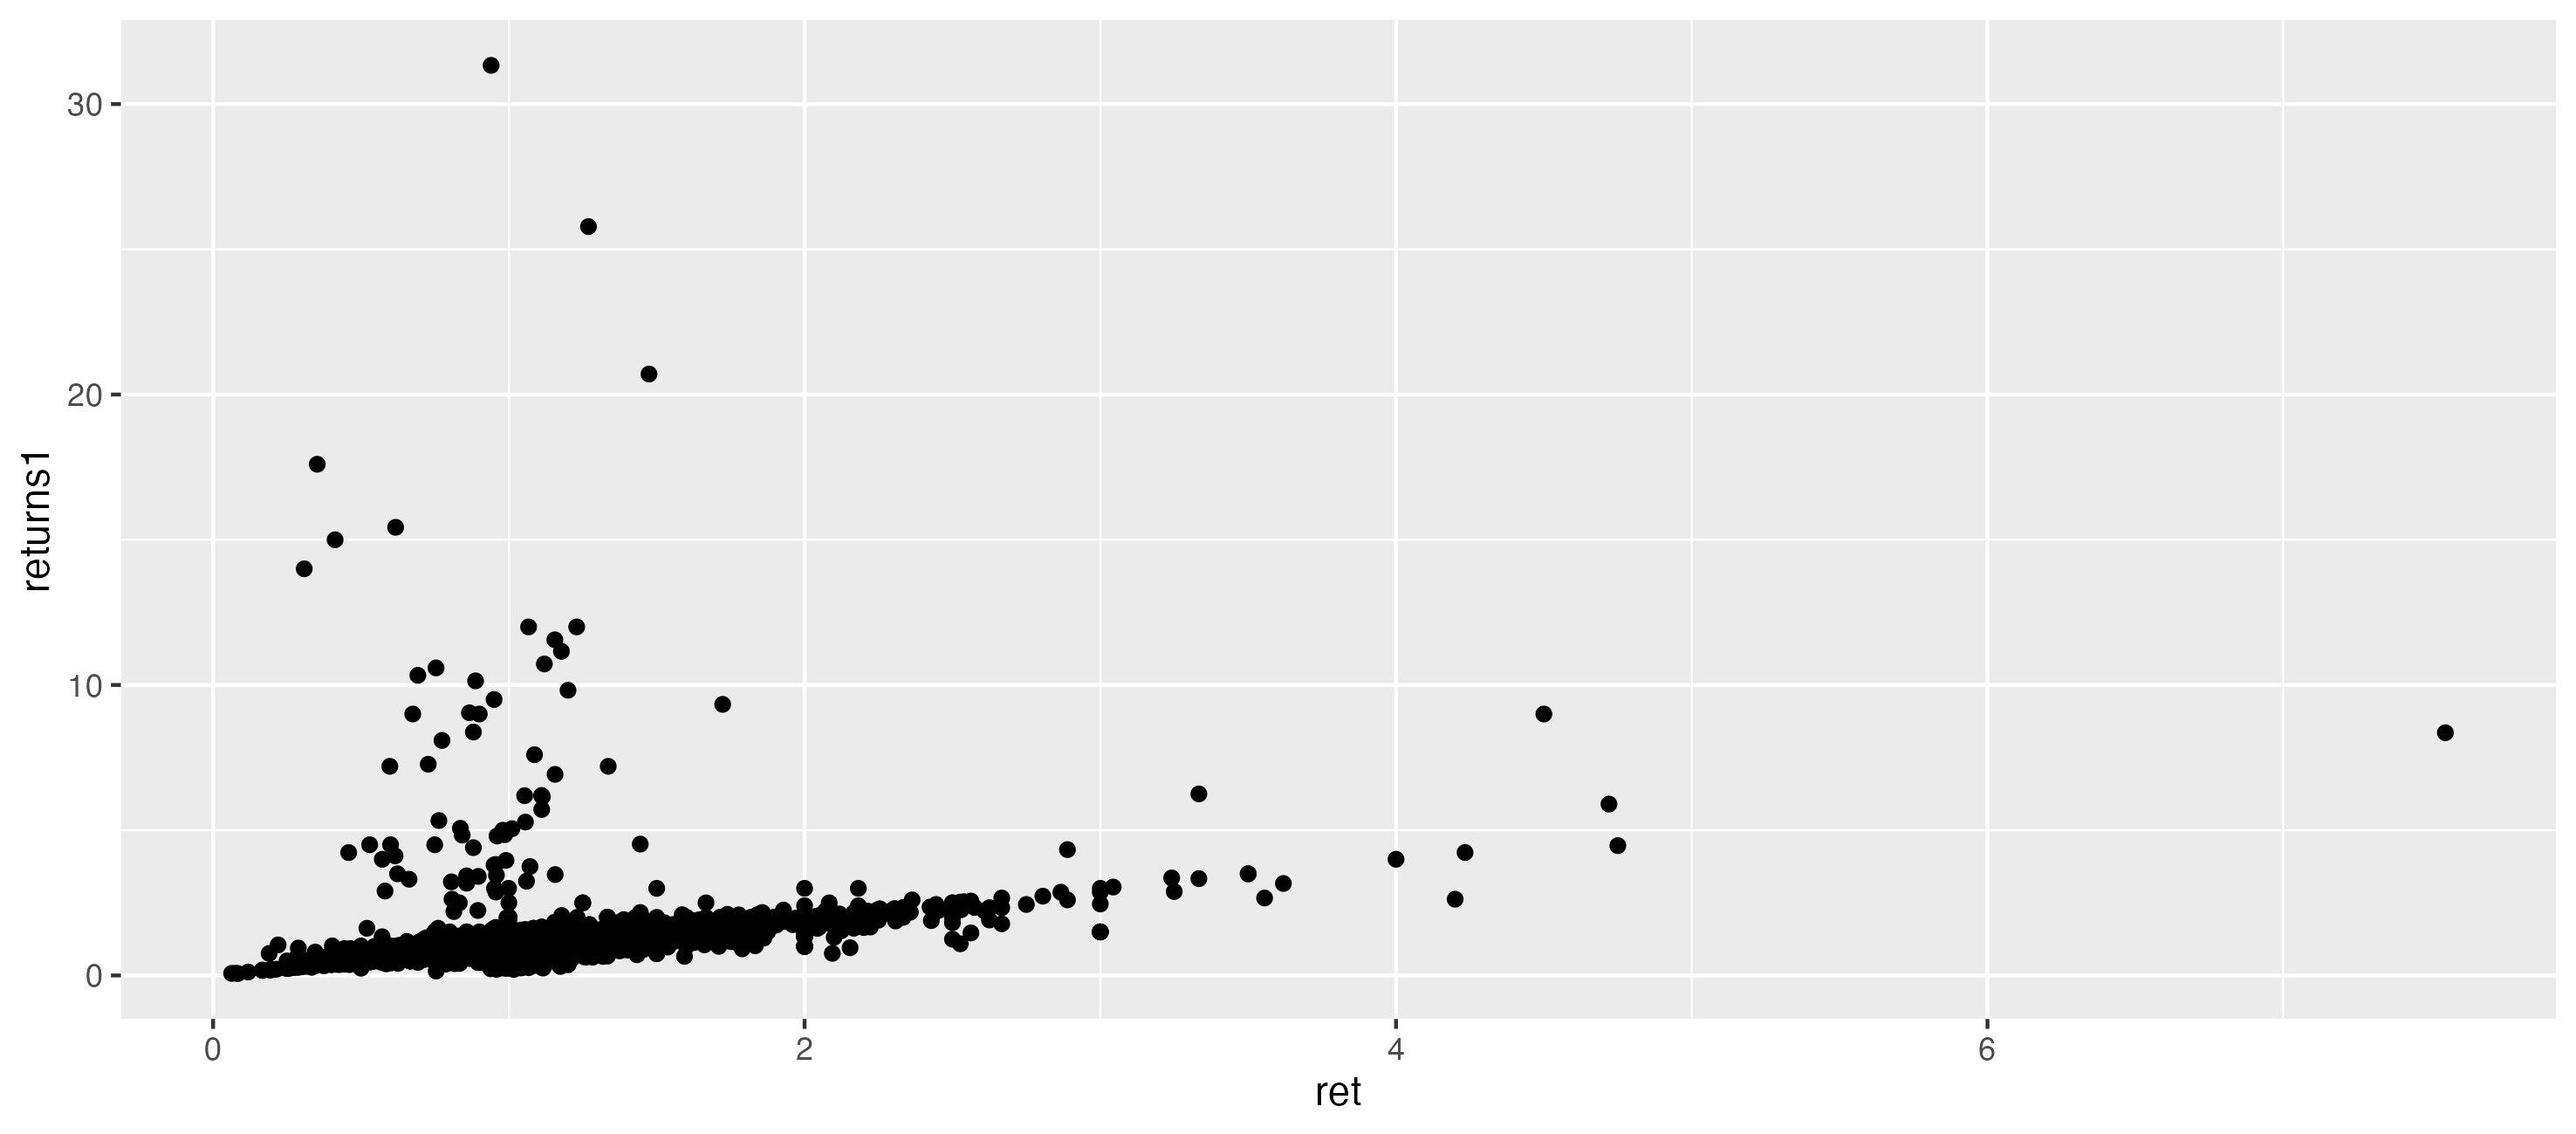
\includegraphics[width=0.45\textwidth]{./Plots/plot_returns_1997.png}} &
		\subfloat[Year 2002]{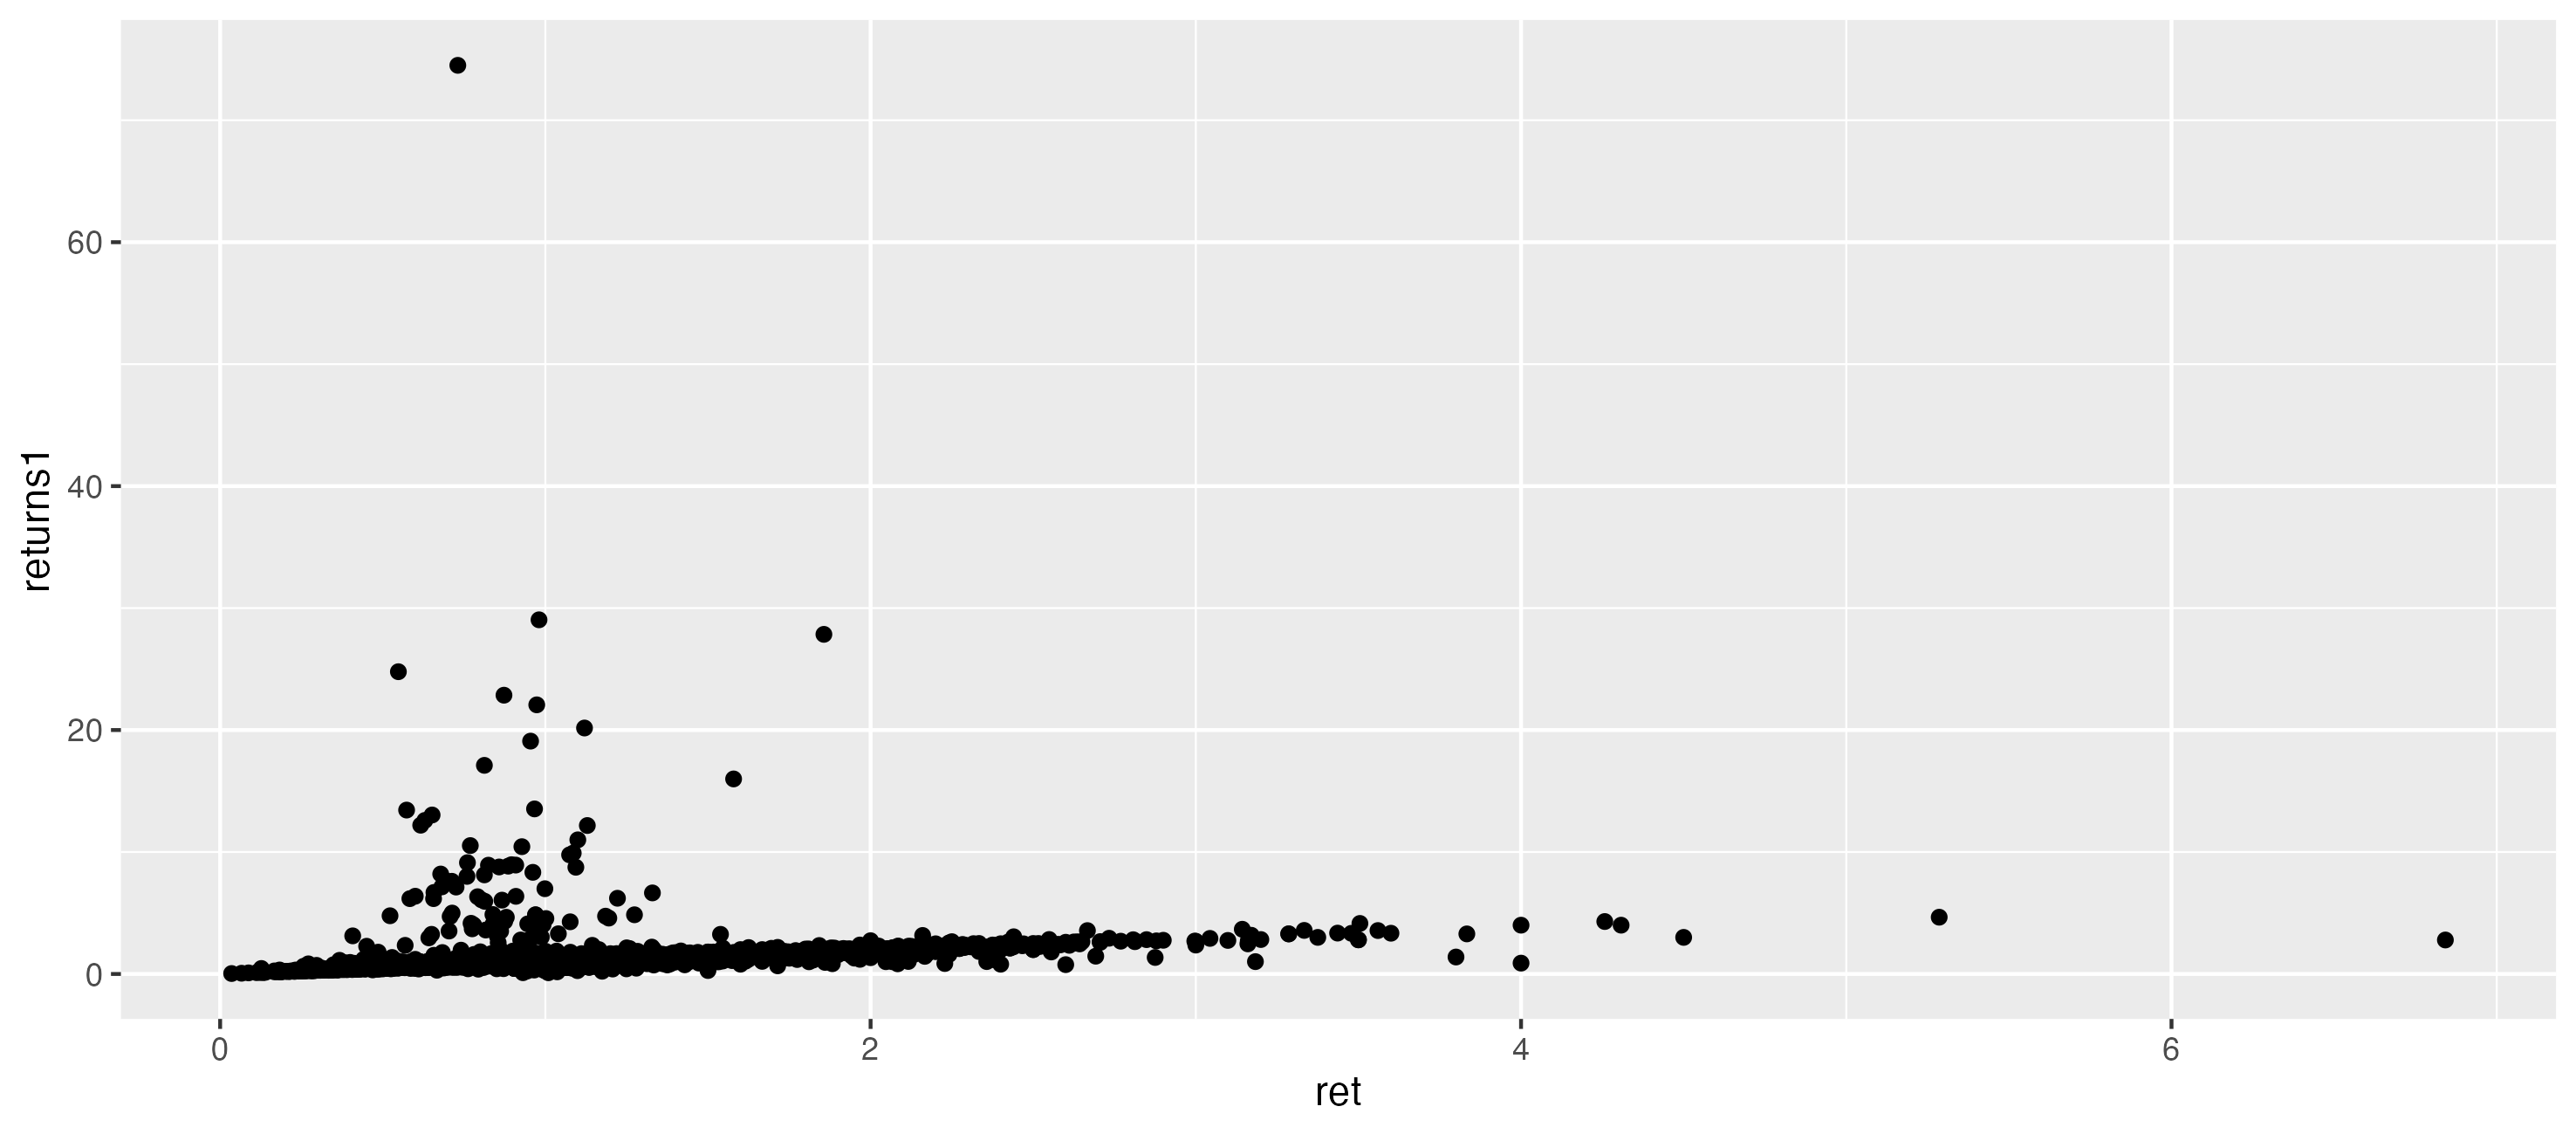
\includegraphics[width=0.45\textwidth]{./Plots/plot_returns_2002.png}} \\
		\subfloat[Year 2006]{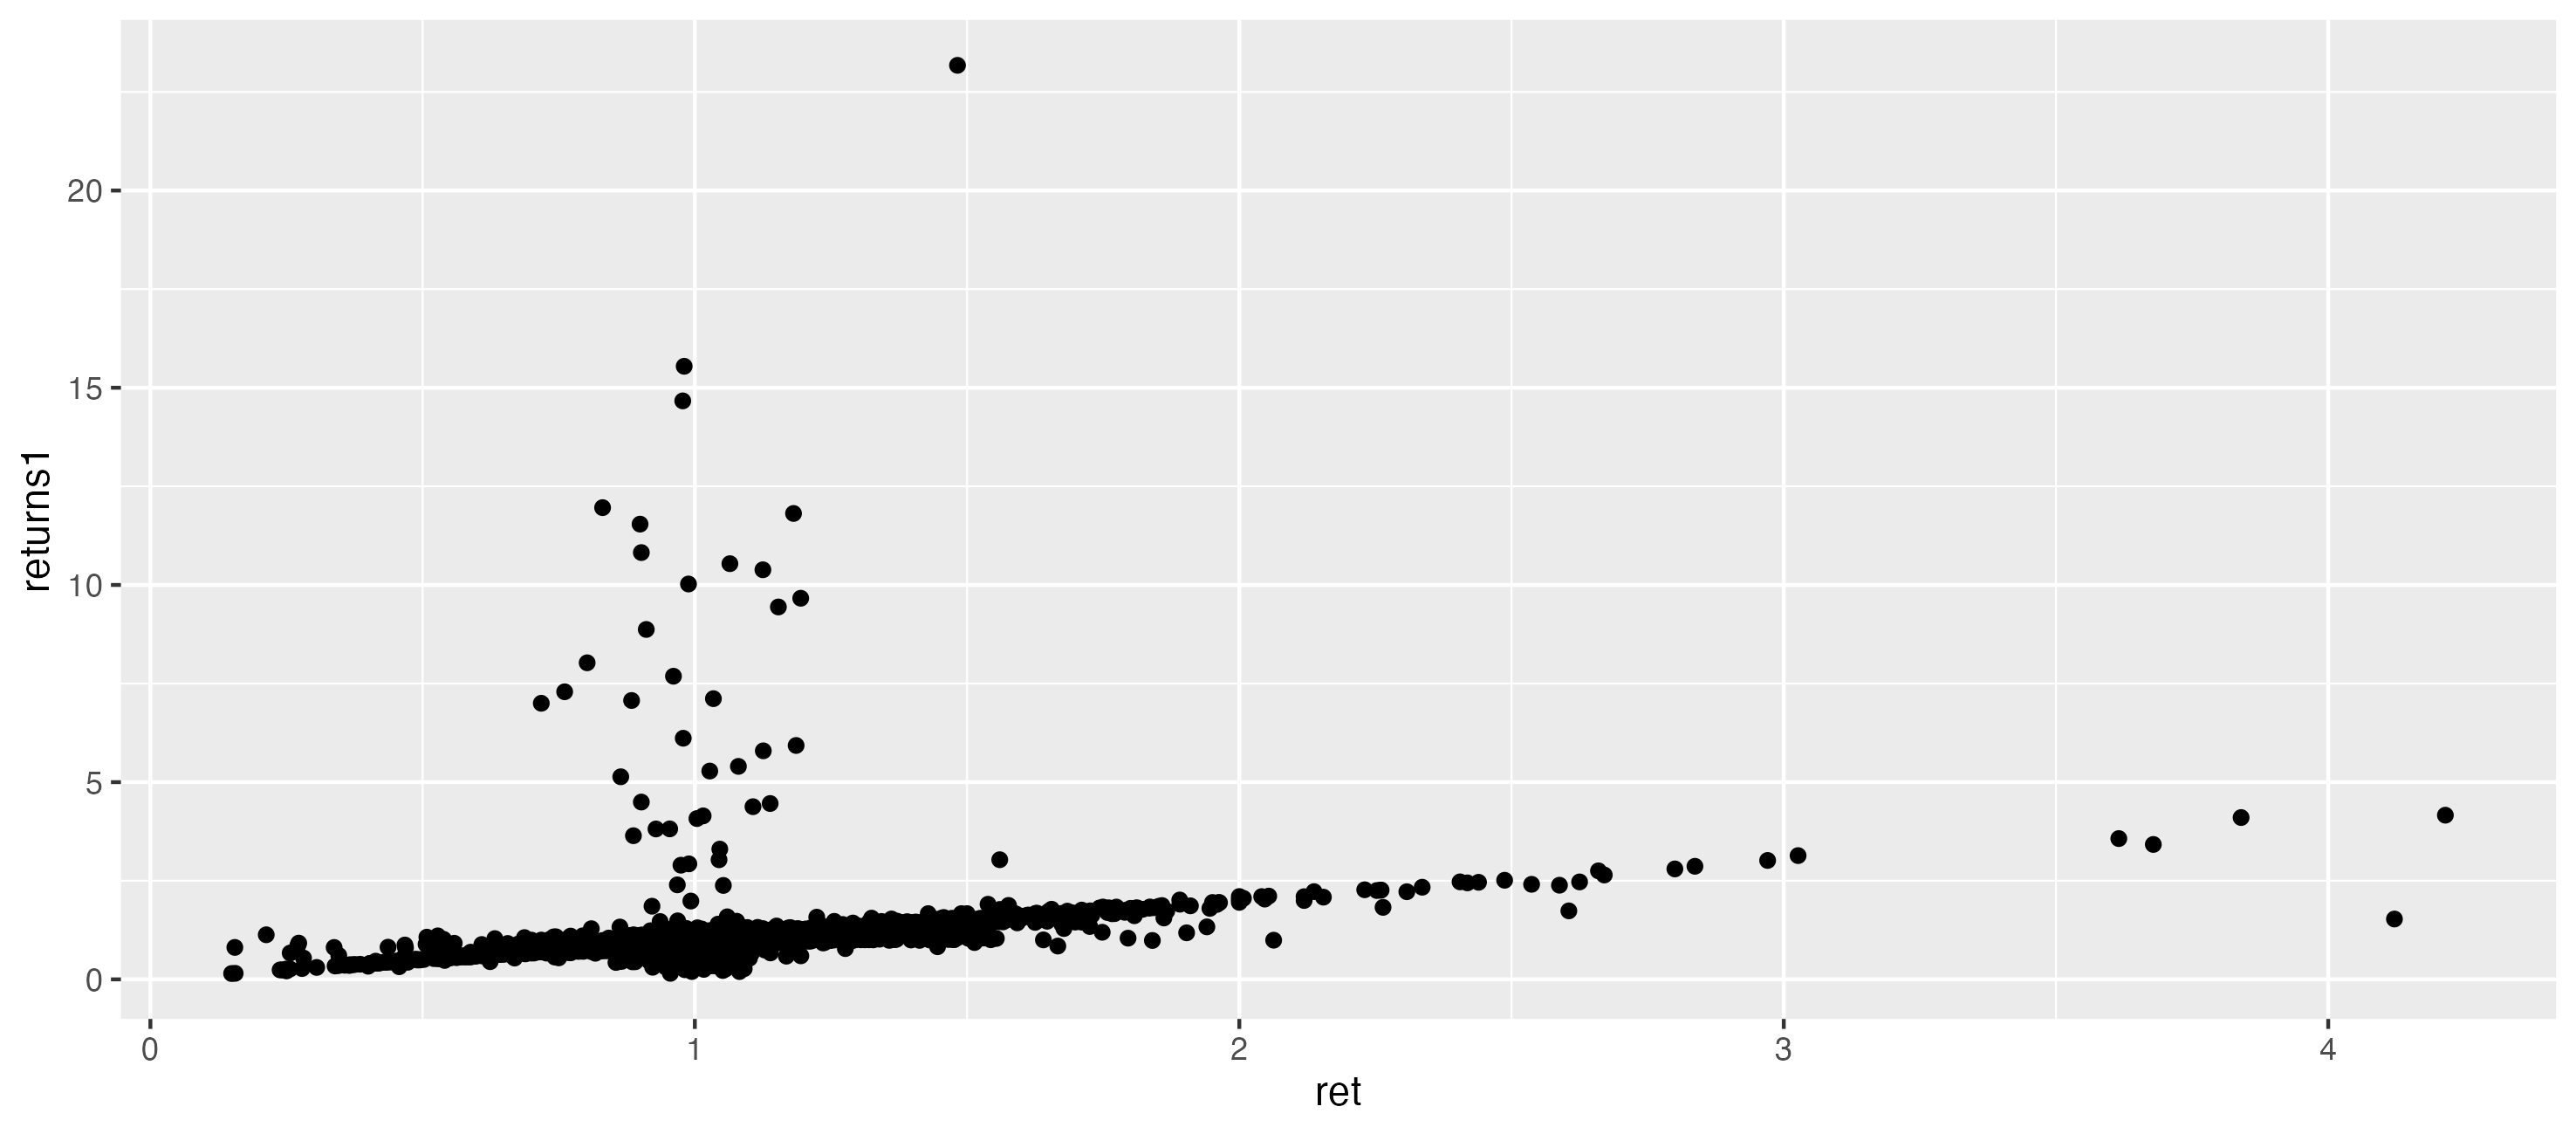
\includegraphics[width=0.45\textwidth]{./Plots/plot_returns_2006.png}} &		\subfloat[Year 2010]{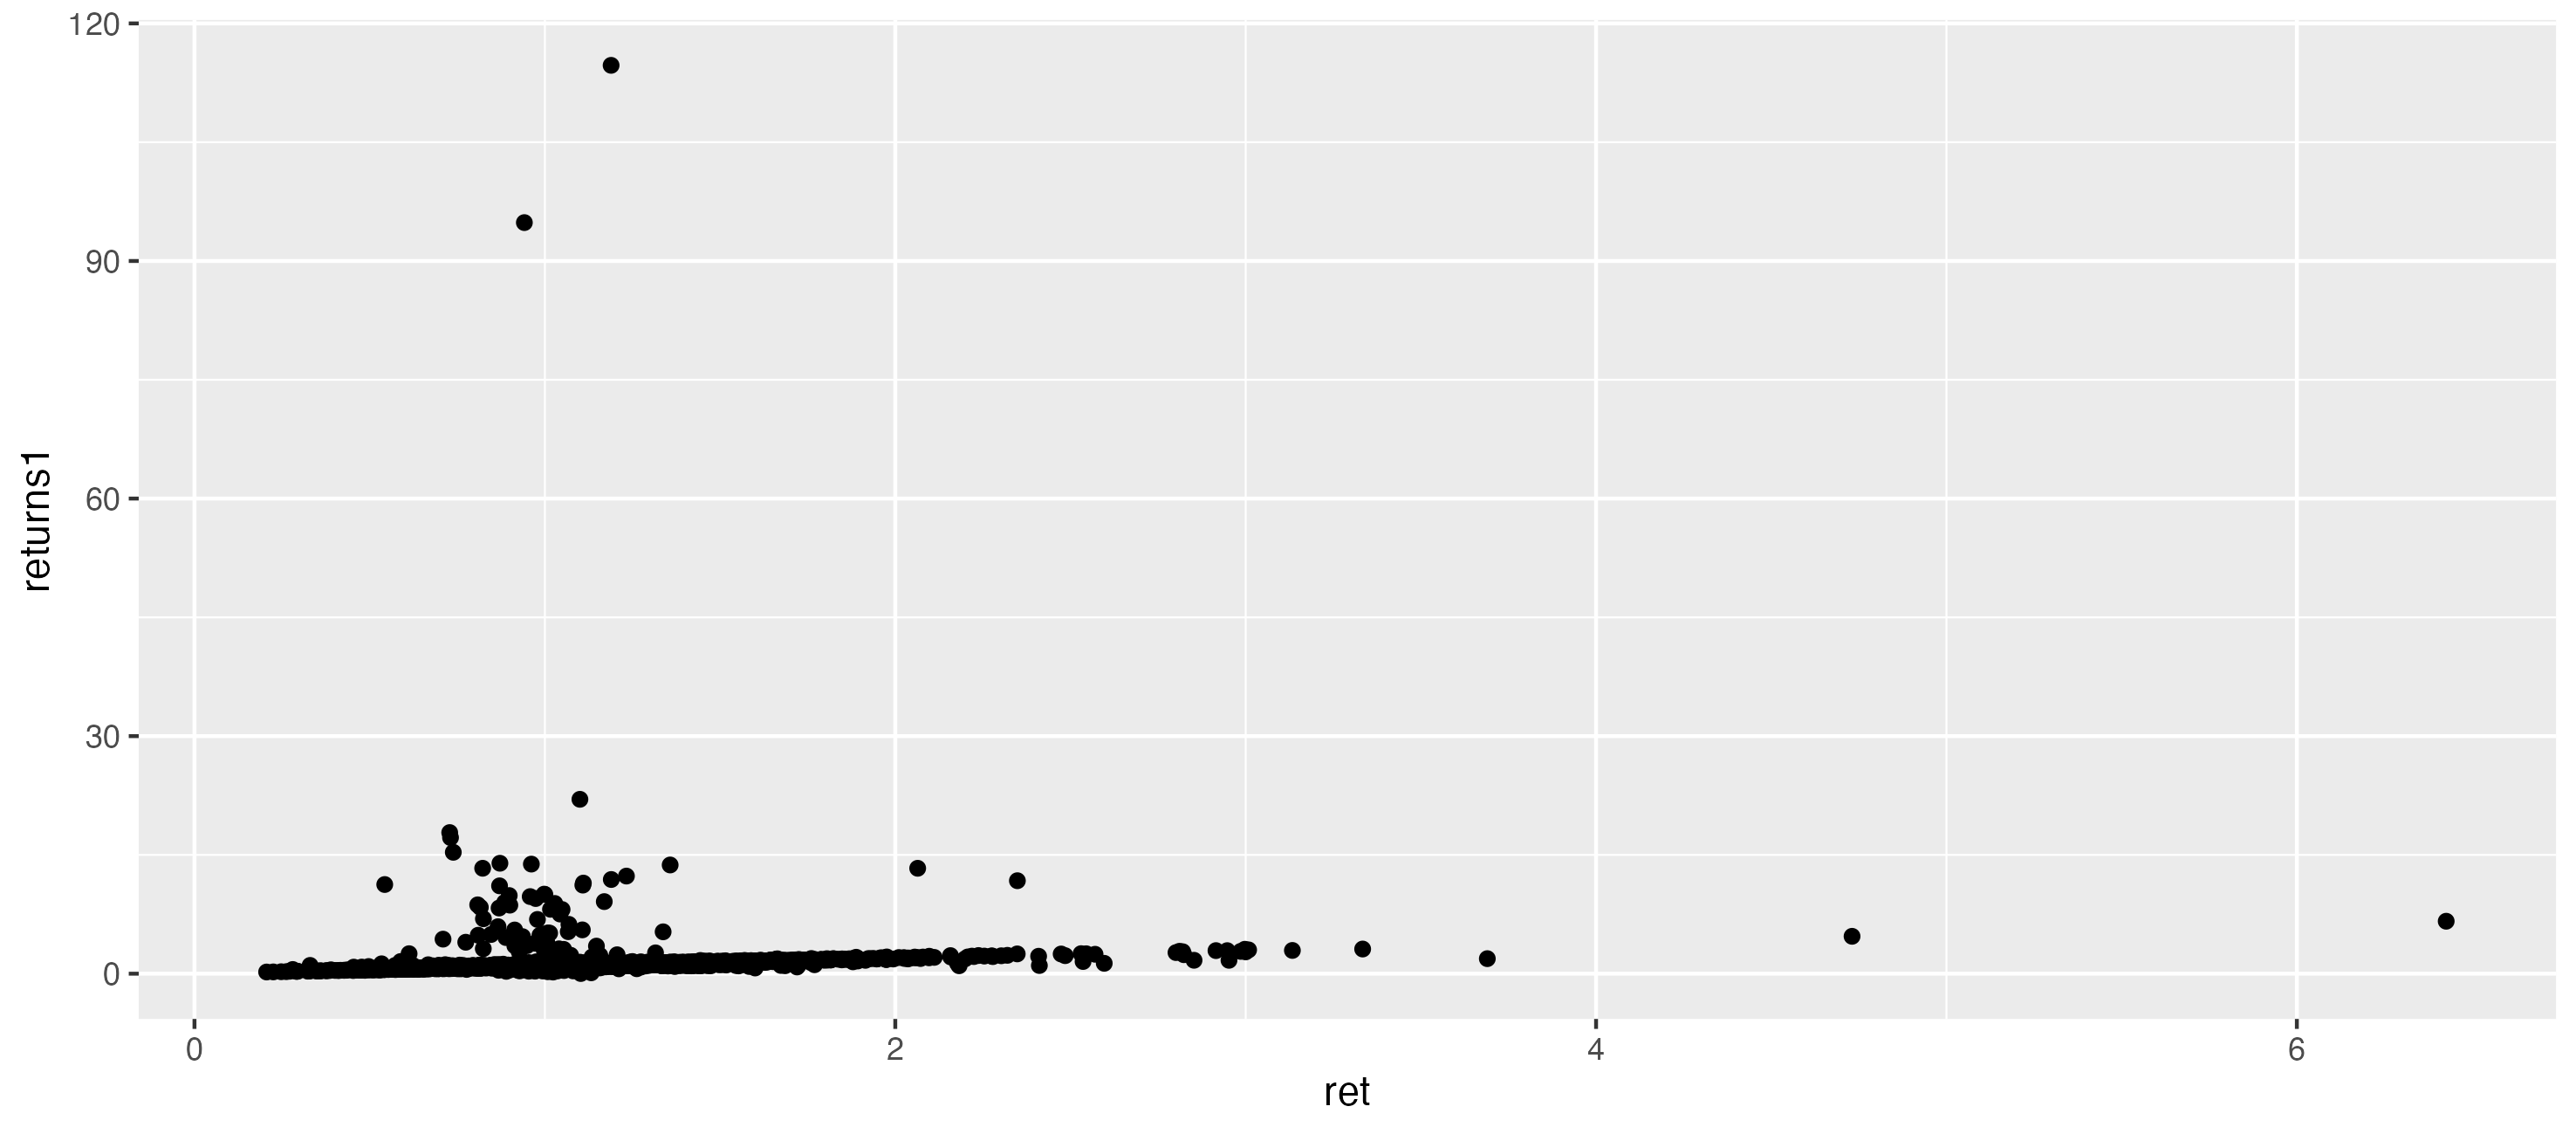
\includegraphics[width=0.45\textwidth]{./Plots/plot_returns_2010.png}} \\
		\subfloat[Year 2015]{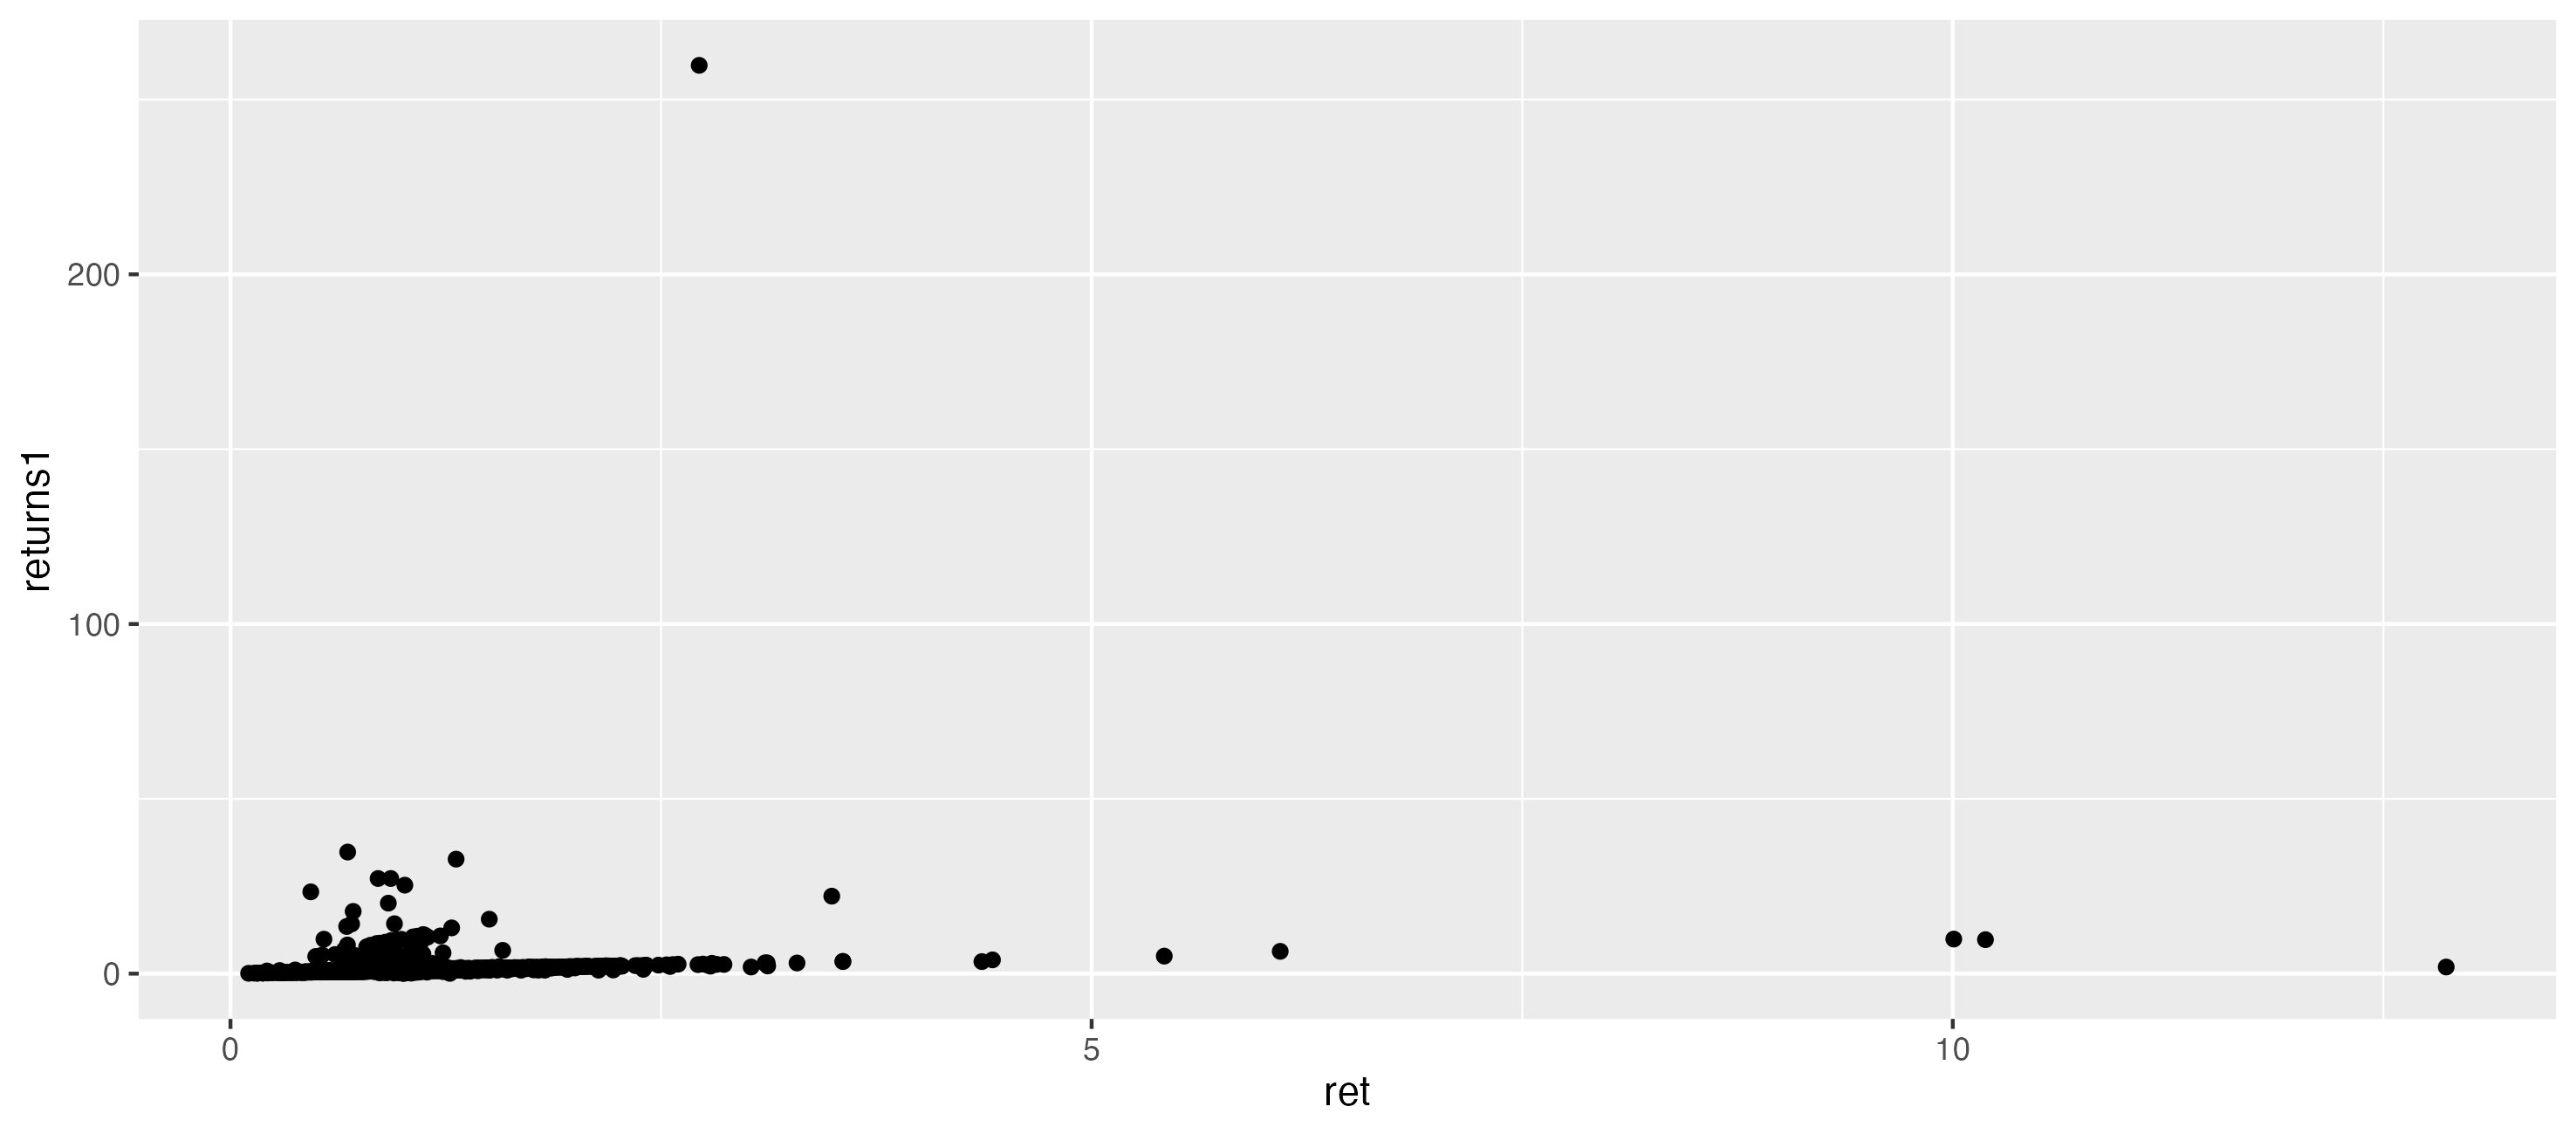
\includegraphics[width=0.45\textwidth]{./Plots/plot_returns_2015.png}} &
		\subfloat[Year 2021]{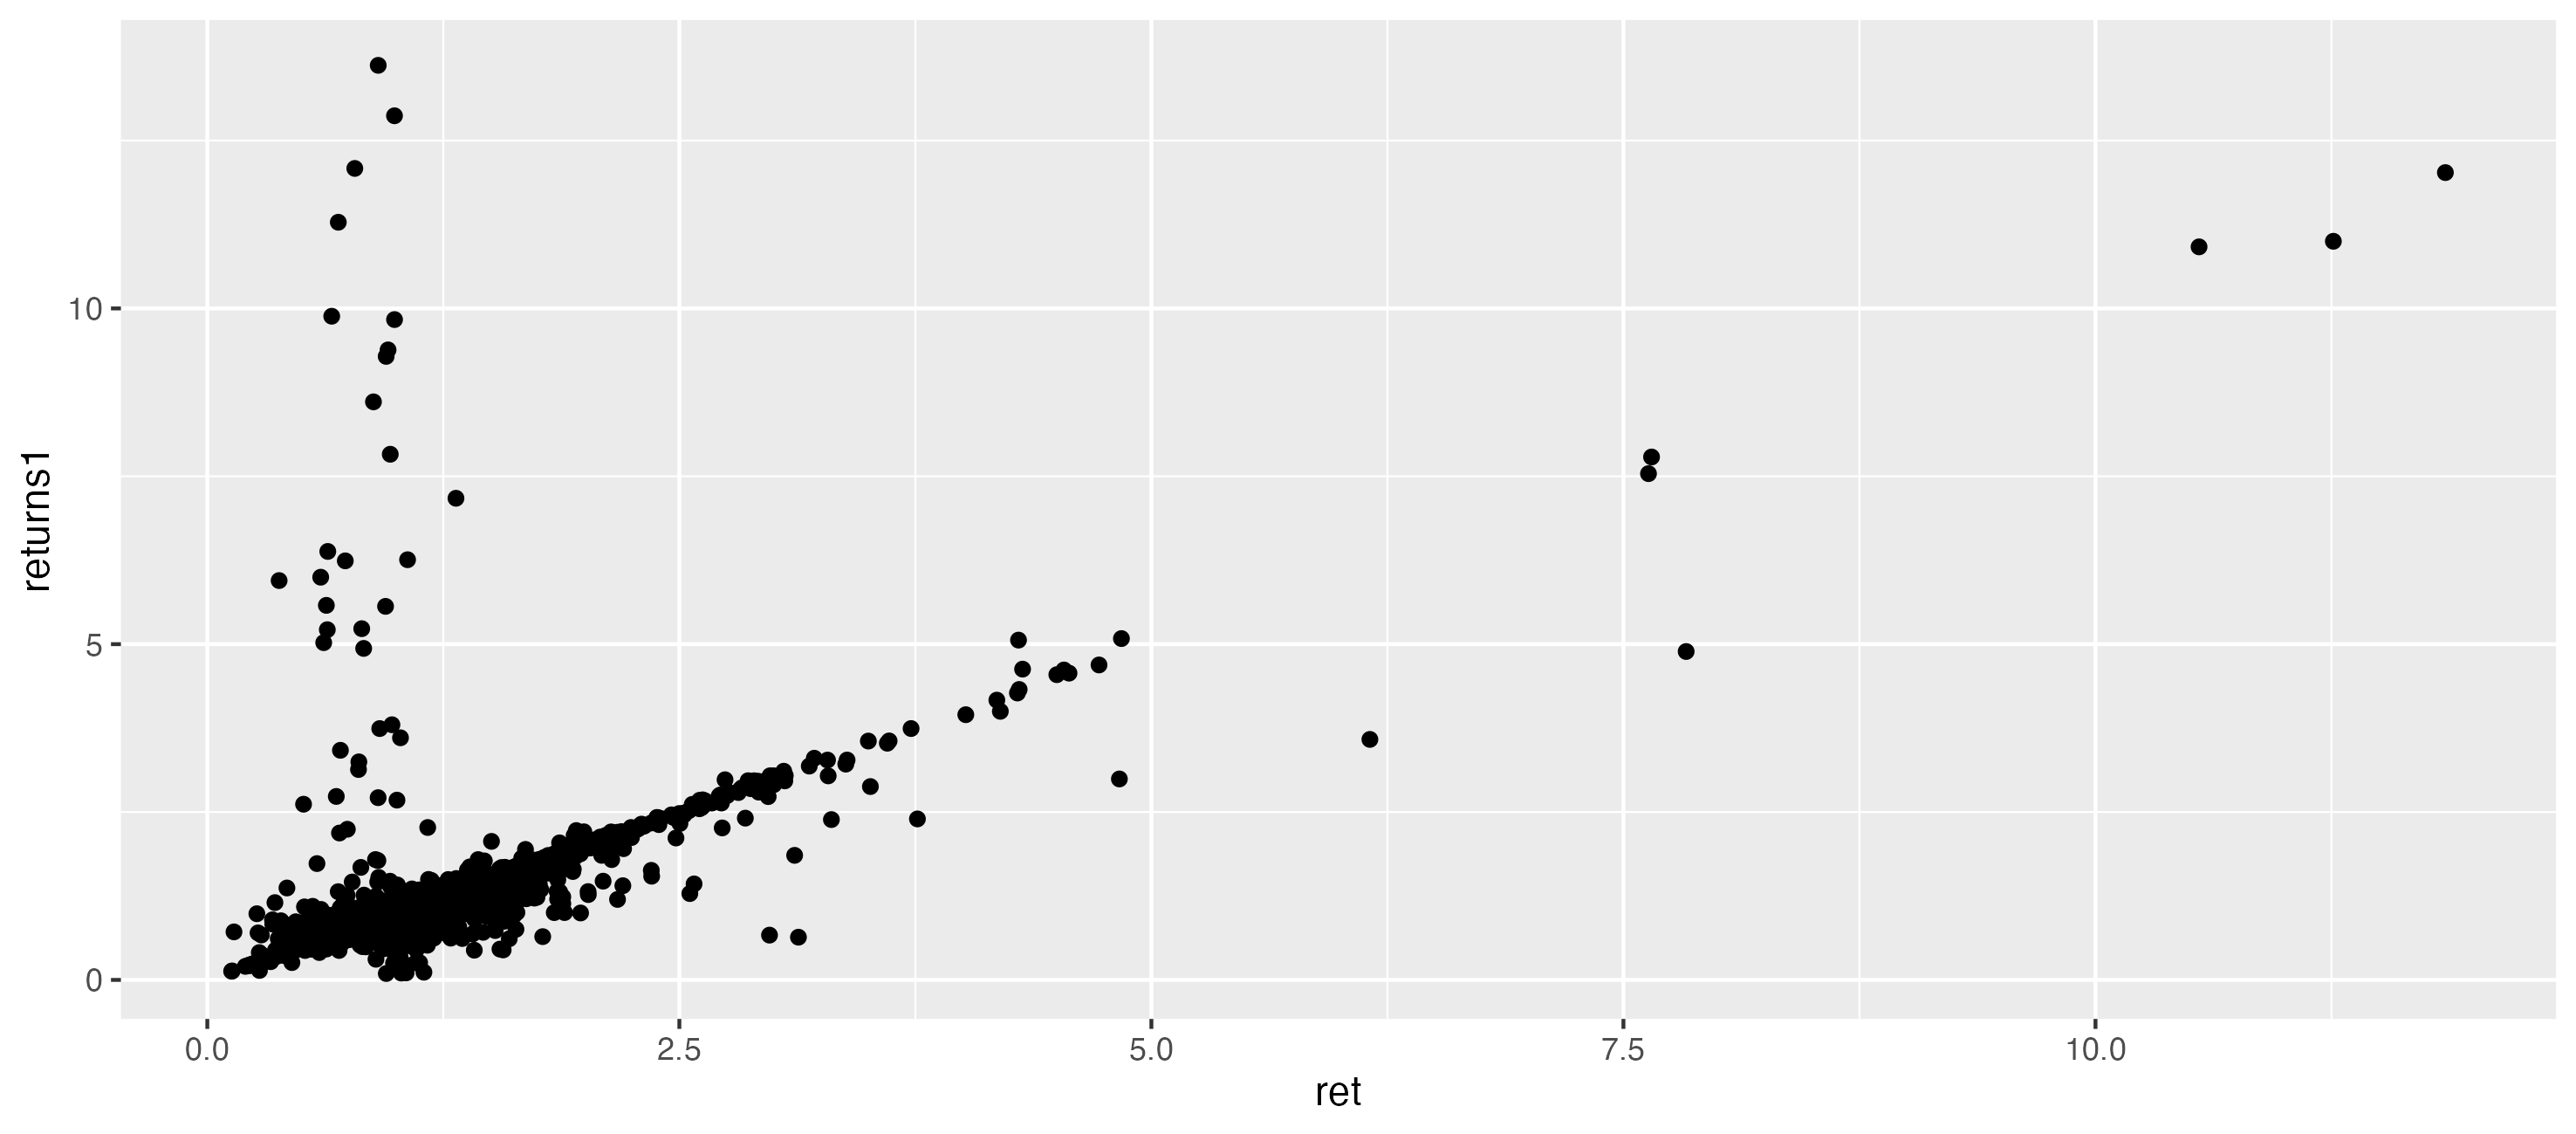
\includegraphics[width=0.45\textwidth]{./Plots/plot_returns_2021.png}} \\
	\end{tabular}
	\label{fig:crspreturns_openclose_vs_ret}
	
	{\small Note: Figure shows the difference between using the daily holding period return supplied by CRSP or calculating the returns as open/close every trading day without accounting for stock splits or dividends, of all returns in the sample across the particular year. The x axis depicts (ret) daily holding return, and the y axis depicts (returns1) open/close. This is just 6 representative years of data evenly spaced out throughout the sample period.}
\end{figure}

\begin{figure}
	\centering
	\caption[Distribution of the Implied Volatility Spread]{Plots of the distribution of the Implied Volatility Spread, across modifications to the signal}
	
	\begin{tabular}{cccc}
		\subfloat[Filtered \& weighted signal]{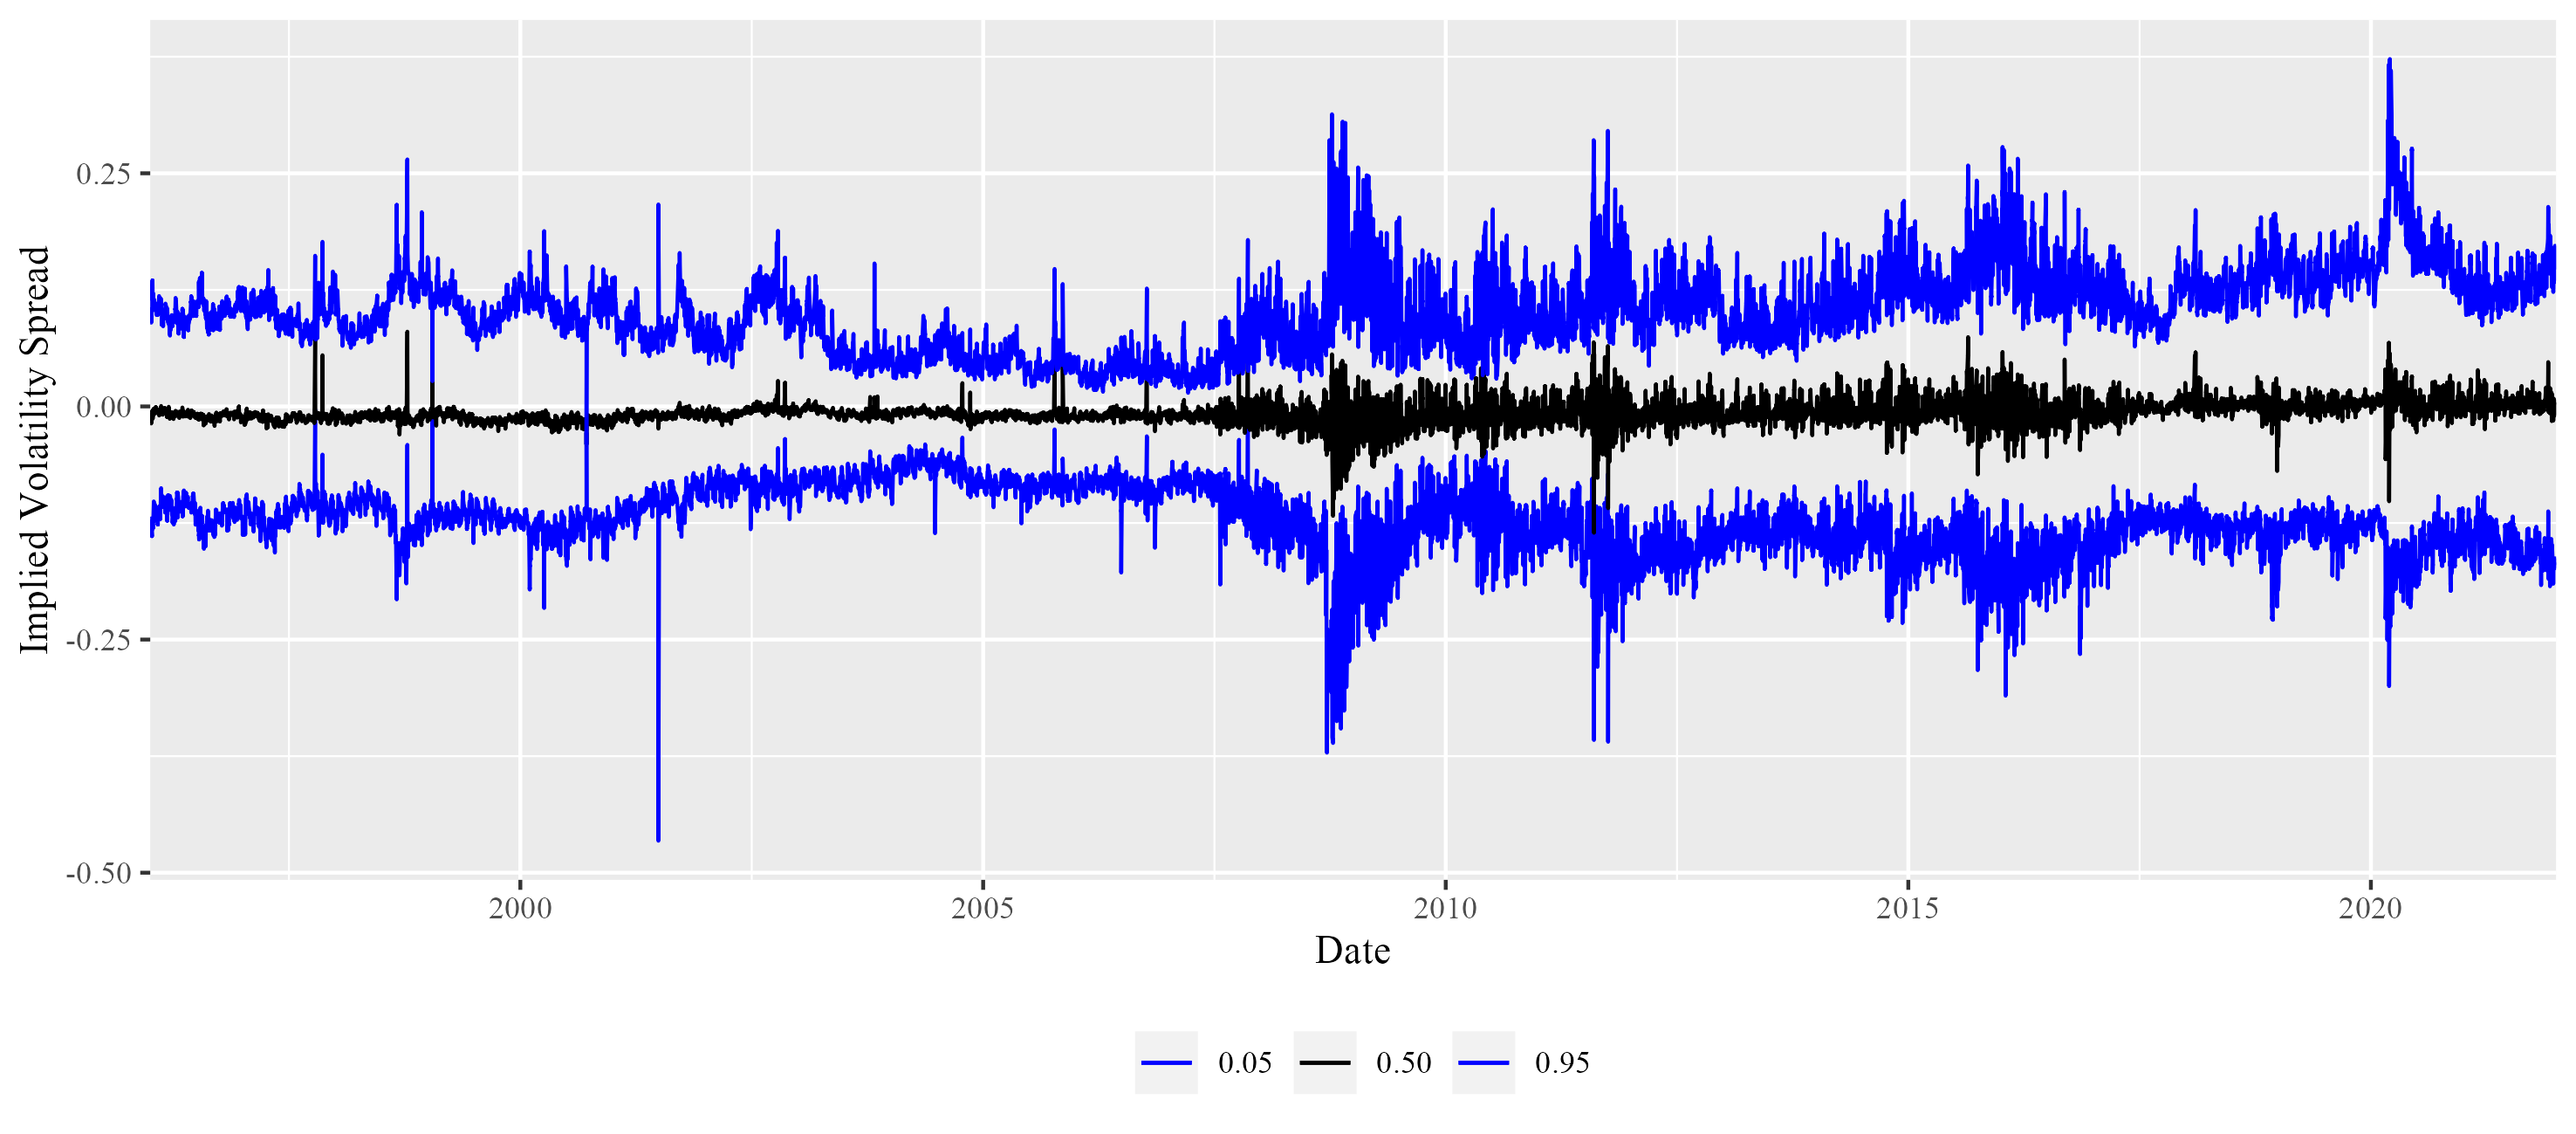
\includegraphics[width=0.6\textwidth]{./Plots/implvolspread_entireperiod_filtered_weighted.png}} \\
		\subfloat[Raw \& weighted signal]{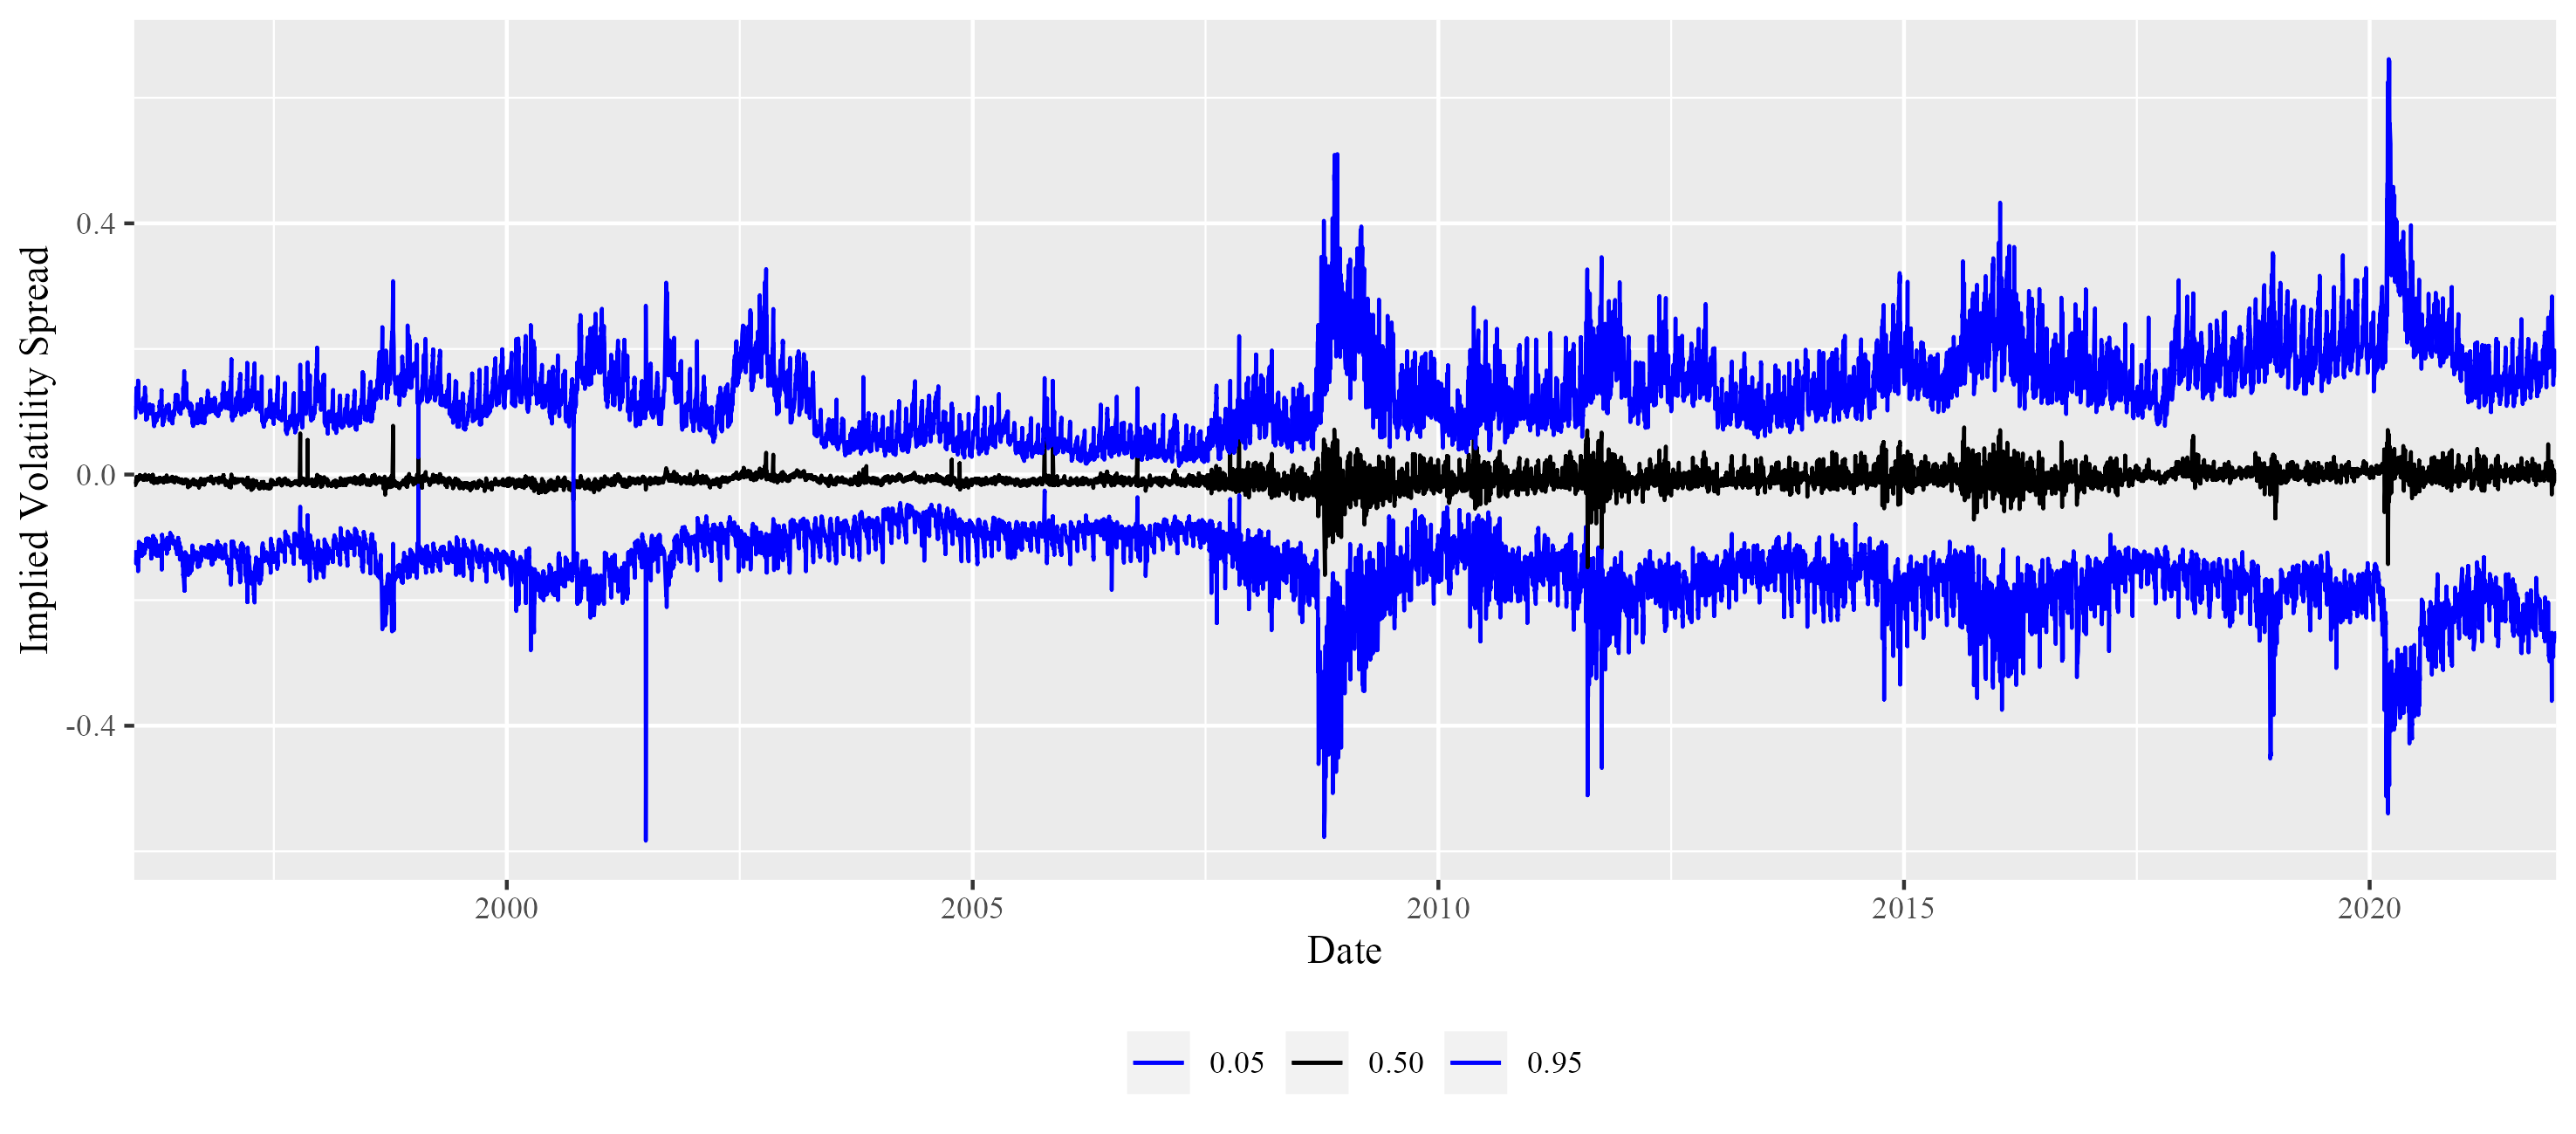
\includegraphics[width=0.6\textwidth]{./Plots/implvolspread_entireperiod_raw_weighted.png}} \\
		\subfloat[Filtered \& simple signal]{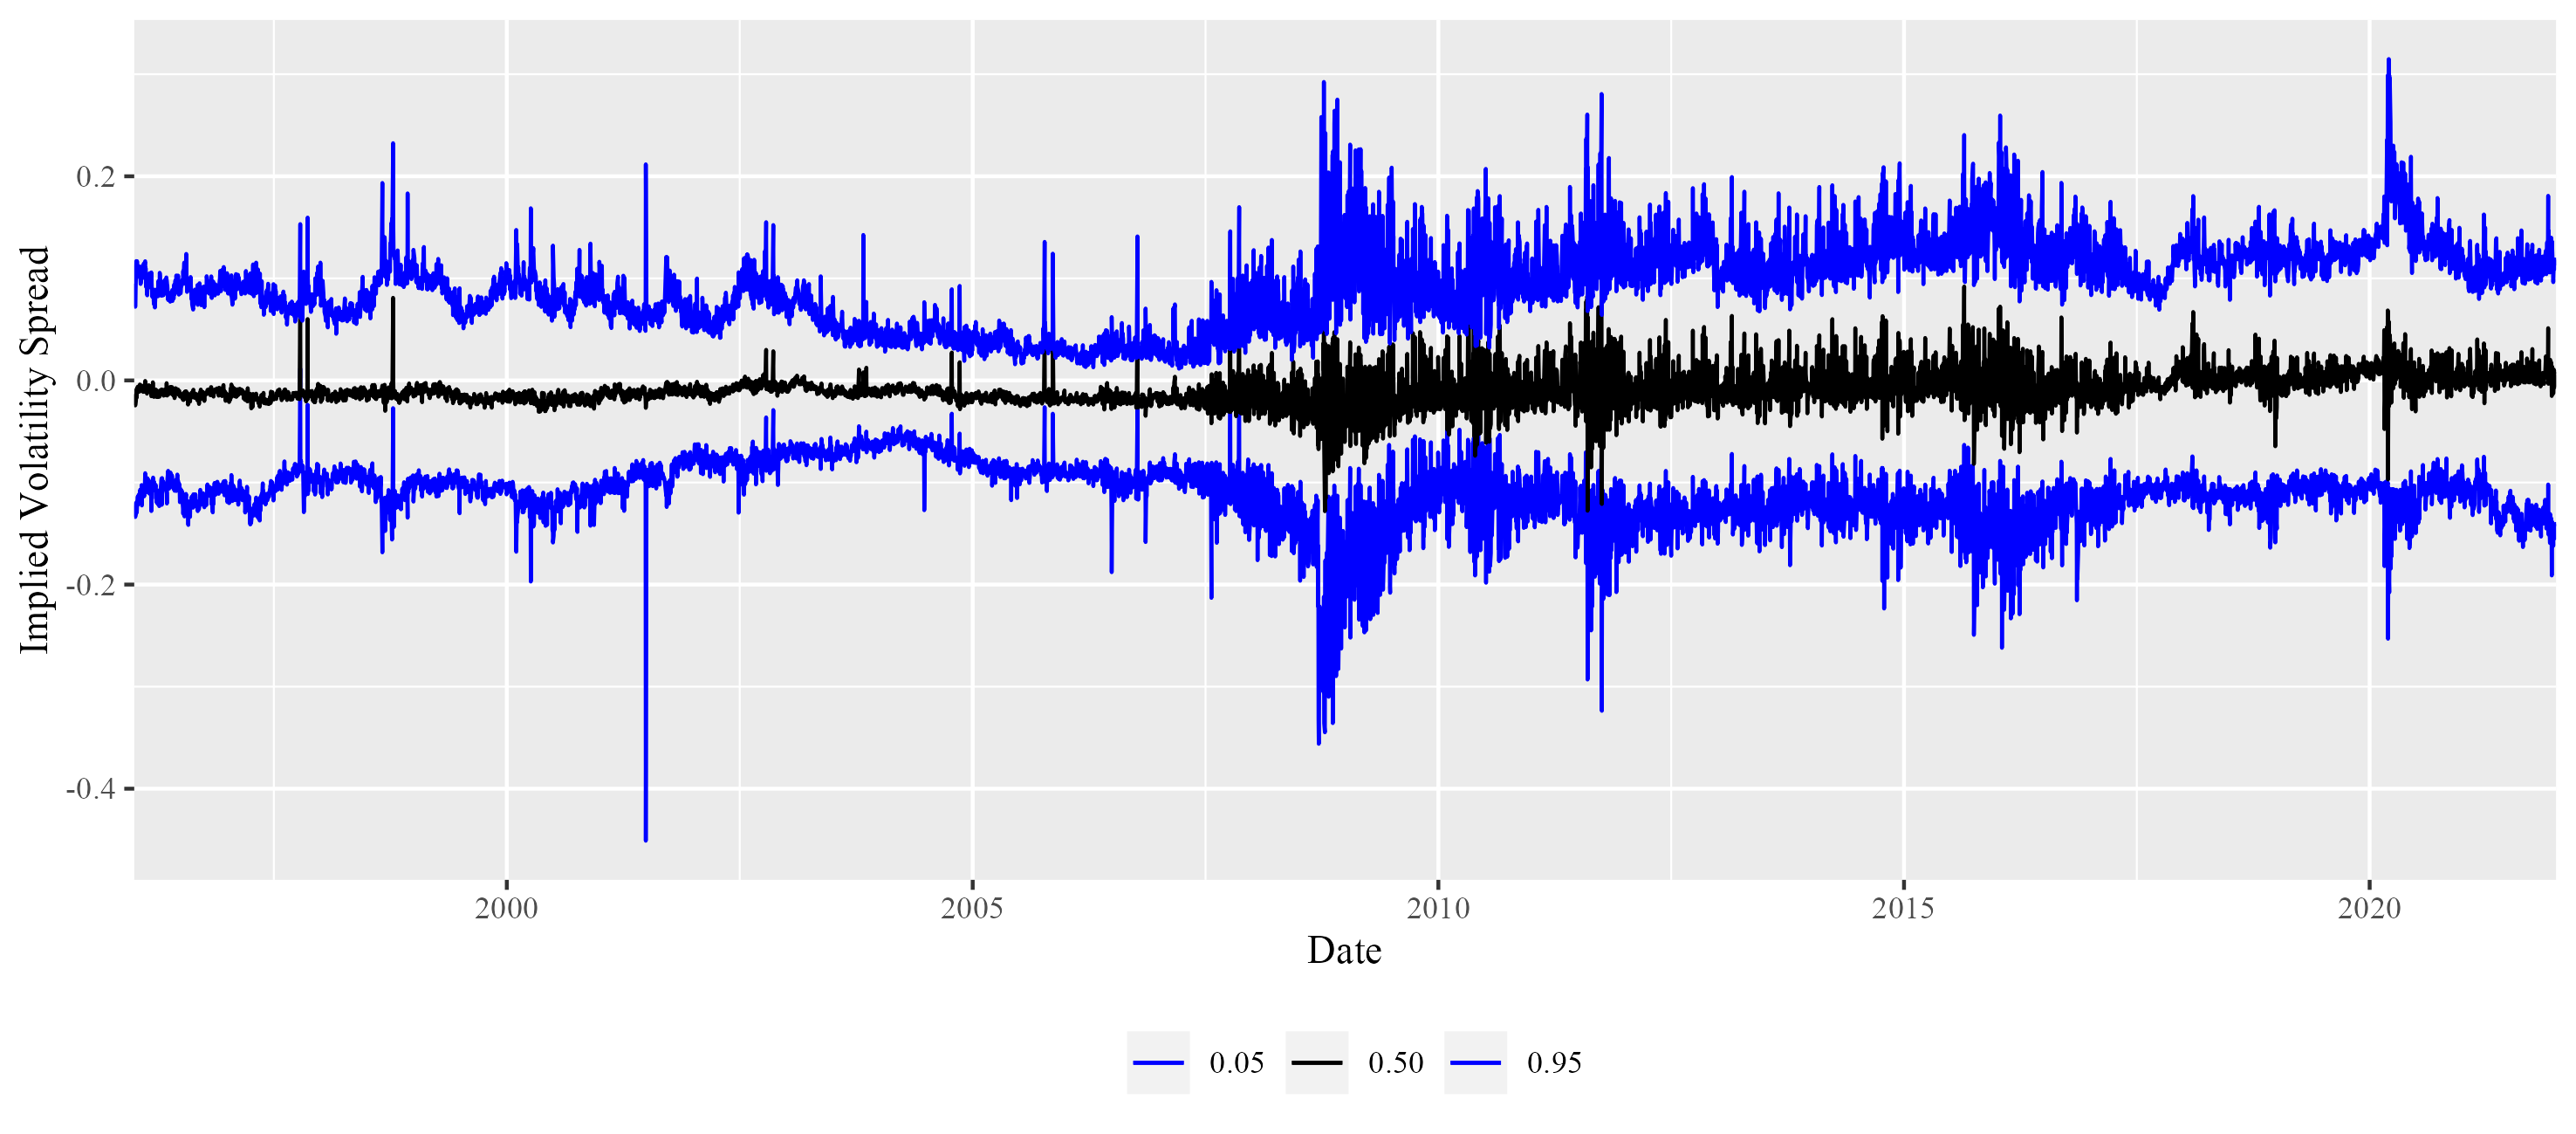
\includegraphics[width=0.6\textwidth]{./Plots/implvolspread_entireperiod_filtered_simple.png}} \\
		\subfloat[Raw \& simple signal]{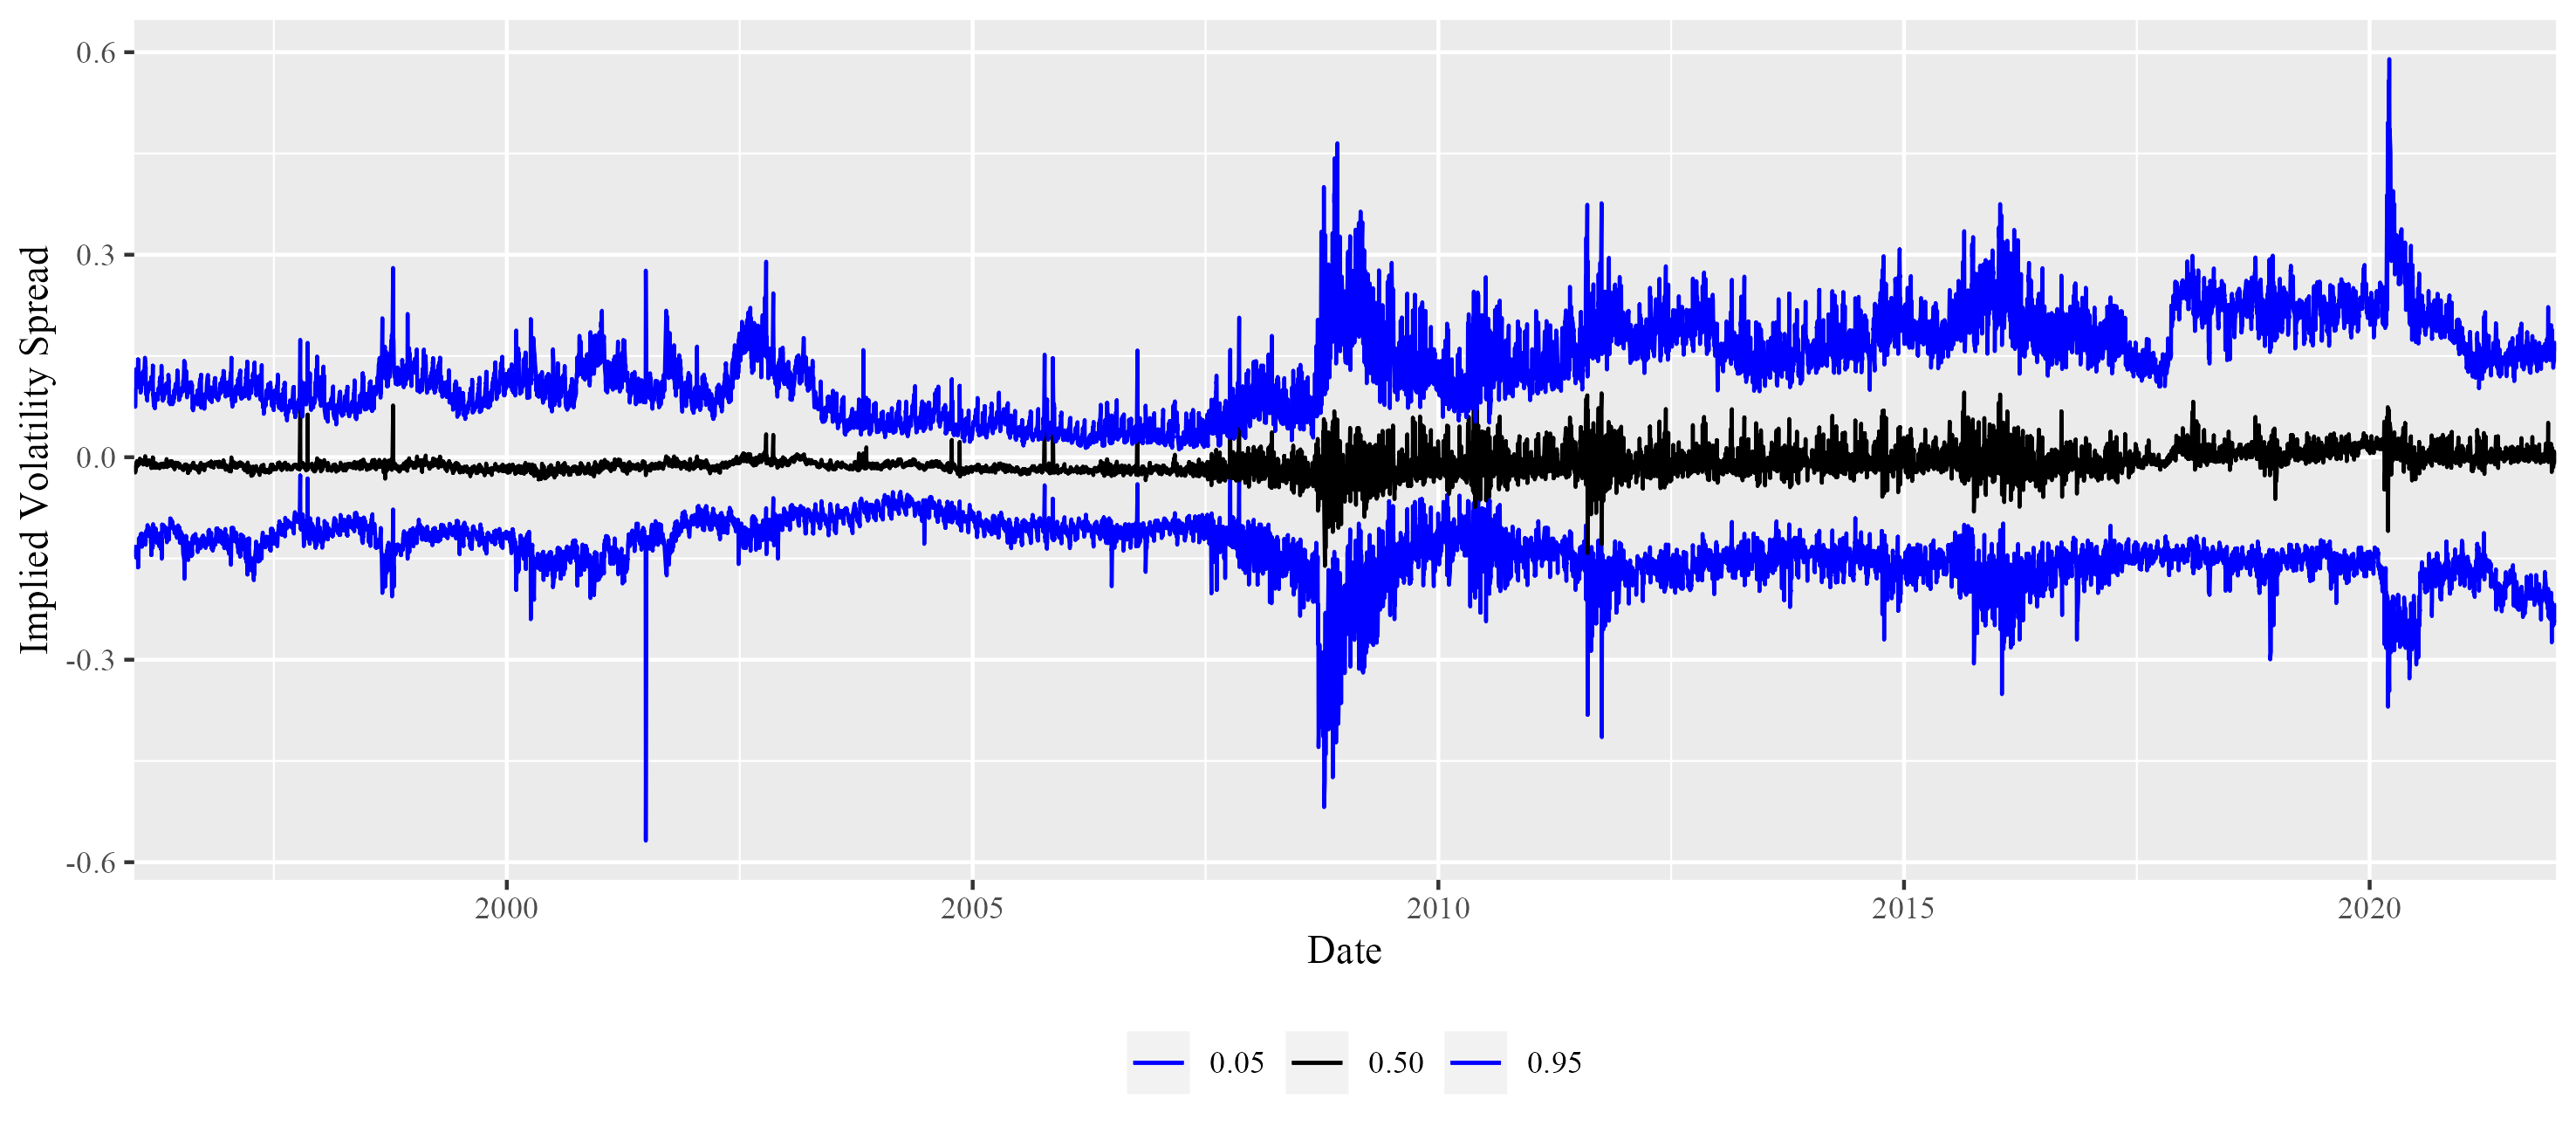
\includegraphics[width=0.6\textwidth]{./Plots/implvolspread_entireperiod_raw_simple.png}} \\
		\end{tabular}
	\label{fig:distribution_of_signal_entire_period}
	
	{\small Note: Figure shows the distribution of the implied volatility spread across the entire sample period. Filtered and raw dictates if the conditions outlined in section \ref{section:data} are implemented. Simple or weighted dictates if the implied volatility spread is weighted by the open interest for each pair. The blue lines are the 0.05 and 0.95 percentiles in the distribution, with the black line equal to the median.}
\end{figure}

\begin{figure}
	\centering
	\caption[ACF of Univariate Portfolio Sort, 5 Implied Vol Spread Level]{Autocorrelation Function of Univariate Portfolio Sort, 5 }
	
	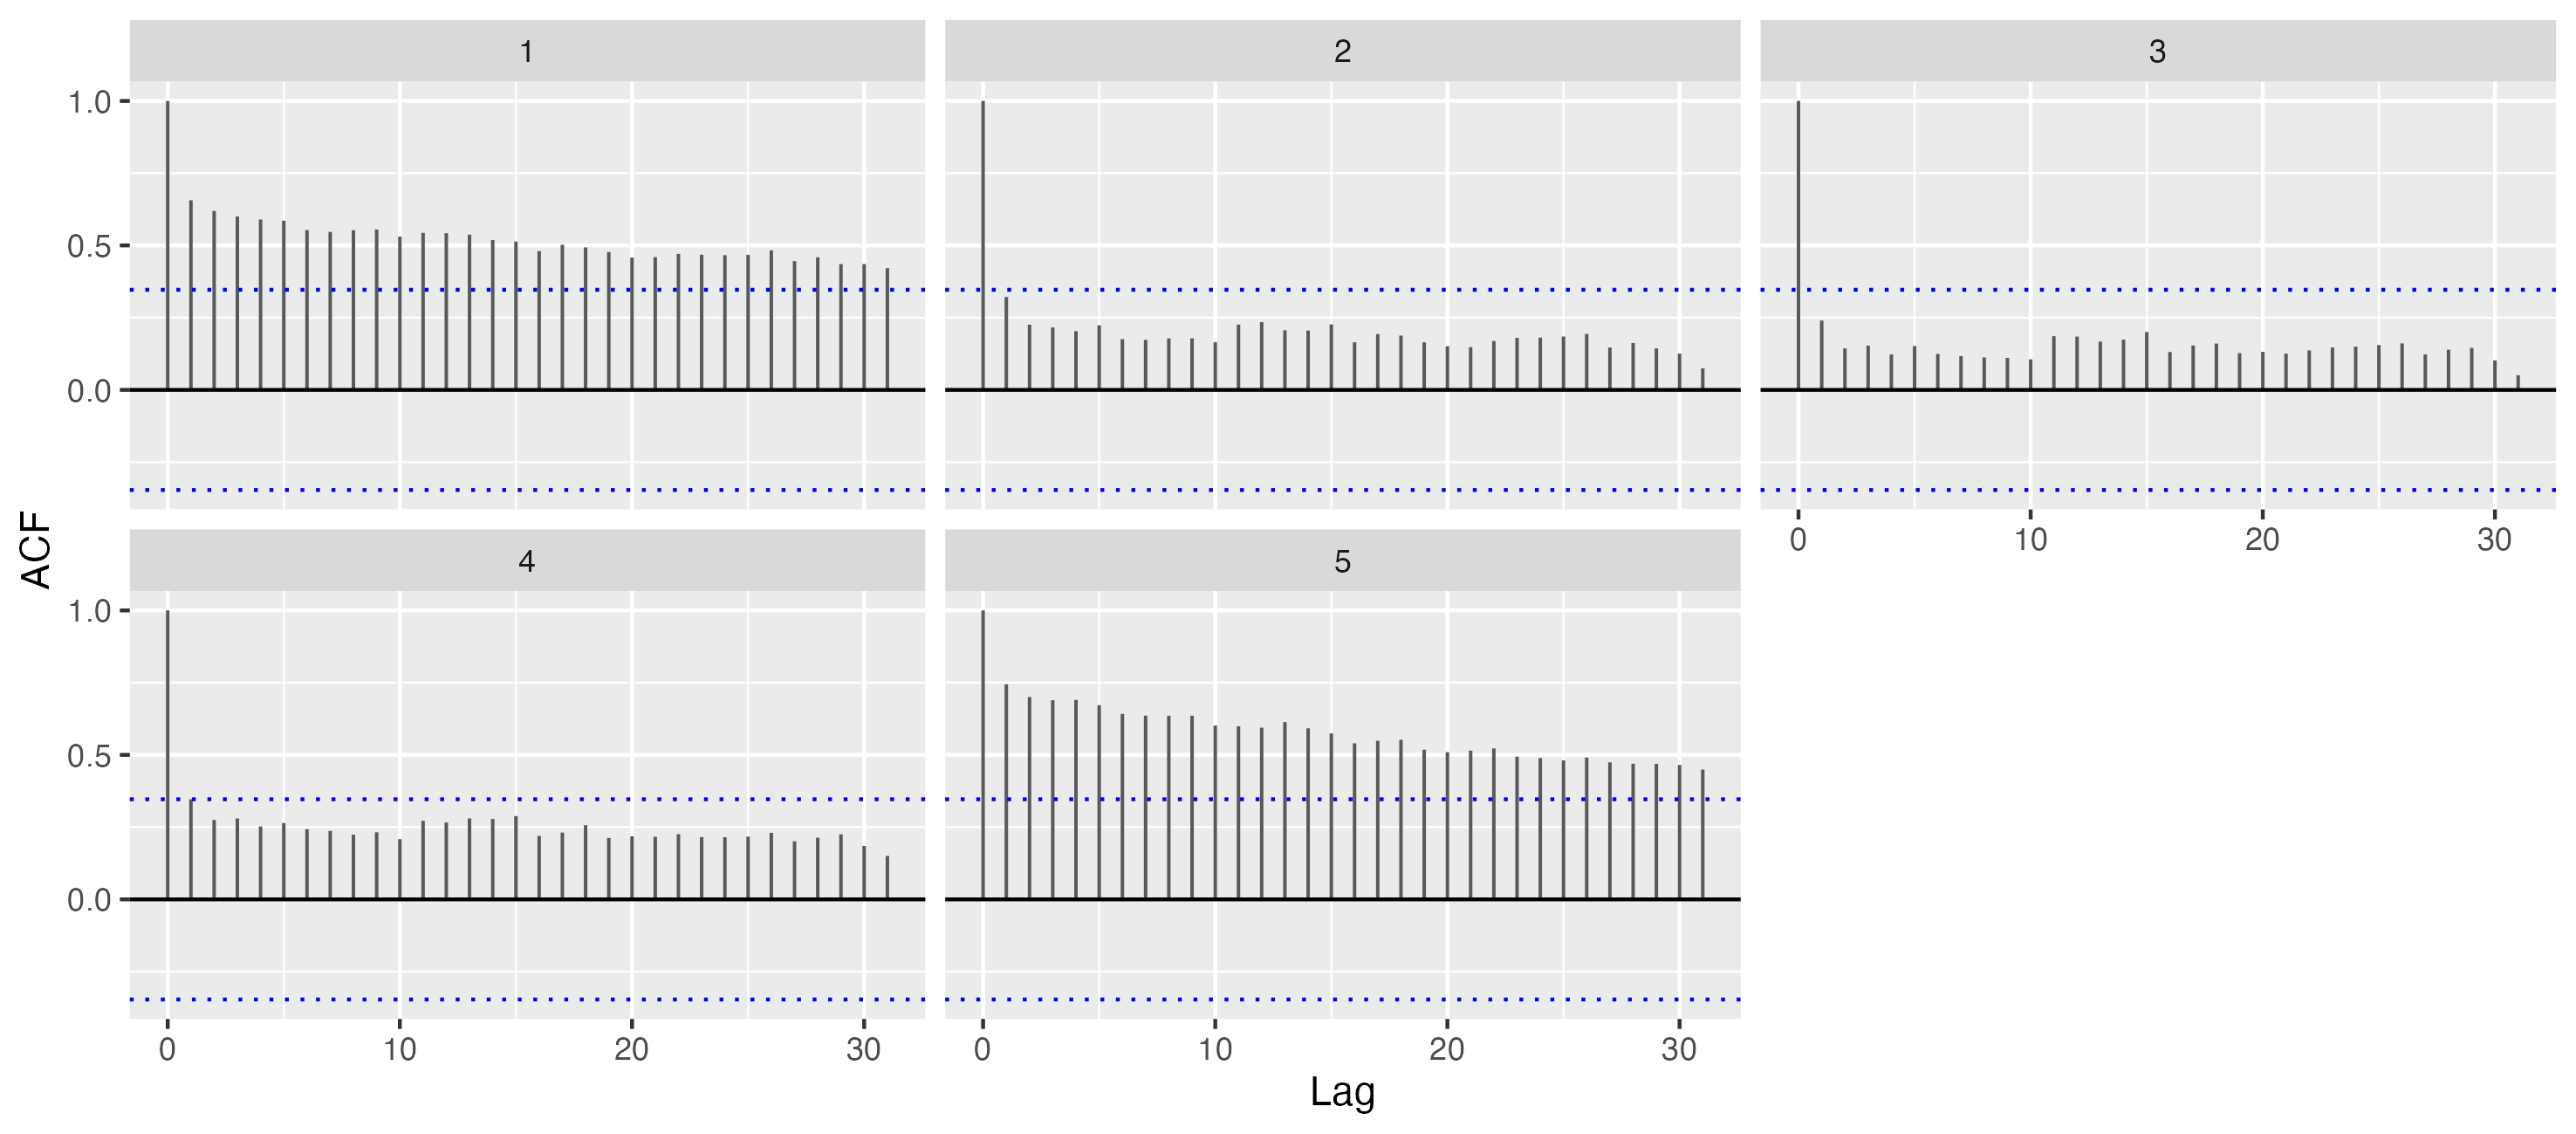
\includegraphics[width=0.95\textwidth]{./Plots/ACF_entireperiod_simple_1.png}
	\label{fig:acf:1}
	
	{\small Note: The five equal-sized portfolios are sorted on the implied volatility spread across the entire sample period with value-weighted weekly returns, with a signal observed on the last trading day before the next week (in which the return is observed) incurred. The returns have been demeaned across t before calculated the ACF.}
	
\end{figure}


\clearpage

%%%%%%%%%%%%%%%%%%%%%%% Appendix B (Math) %%%%%%%%%%%%%%%%%%%%% 
\renewcommand\thesubsection{B}
\subsection{Tables}

\begin{table}[ht]
	{\tiny
	\centering
	\caption[Factor Competition, all factors]{Factor Competition Coefficients, Bivariate Dependent Sort 10x10}
	\label{tab:factor_competition_9_ALL}	
	\begin{tabular}{l|lllllllllllllll}
		% Fri May 26 01:36:58 2023
Dep. Variable & Intercept & Factor & Factor\_D & MKT\_RF & SMB & HML & RMW & CMA \\
  \hline
Factor & 0.97  (***) &  & 0.04 & 0 & -0.02 & 0.09 & -0.11 & -0.04 \\
Factor\_D & 0.49  (***) & 0.03 &  & 0.06 & 0.08 & -0.04 & 0.25  (**) & 0.14 \\
  MKT\_RF & 0.23  (***) & 0 & 0.02 &  & 0.13  (**) & 0.28  (***) & -0.52  (***) & -0.48  (***) \\ 
  SMB & 0.04 & 0 & 0.01 & 0.04  (**) &  & -0.07  (**) & -0.31  (***) & 0.04 \\ 
  HML & -0.05 & 0.01 & -0.01 & 0.11  (***) & -0.09  (**) &  & 0.16  (***) & 0.53  (***) \\ 
  RMW & 0.05 & -0.01 &  0.02  (**) & -0.11  (***) & -0.2  (***) & 0.09  (***) &  & 0.17  (***) \\ 
  CMA & 0.05 & 0 & 0.01 & -0.07  (***) & 0.02 & 0.18  (***) & 0.11  (***) &   \\ 
  BetaLiquidityPS & 0.06 & -0.05  (*) & 0.03 & 0.06 & 0.16  (**) & -0.06 & -0.04 & 0.2  (*) \\ 
  betaVIX & 0.04 &  0.05  (*) & -0.04 & 0.01 & -0.33  (***) & -0.09 & 0.31  (***) & -0.16 \\ 
  CoskewACX & 0.26  (**) & 0.01 & -0.02 & 0.07  (*) & 0.03 & 0.08 & 0.11 & -0.03 \\ 
  Coskewness & 0.1 &  0.03  (*) & -0.02 & 0.03 & -0.15  (***) & 0 & -0.07 & -0.26  (***) \\ 
  OptionVolume1 & 0.46  (***) & 0.01 & 0.01 & -0.05 & 0 & 0.23  (***) & 0.29  (***) & 0.26  (***) \\ 
  OptionVolume2 & -0.1 & 0.01 & 0.04  (*) & 0.03 & 0.05 & -0.14  (**) & -0.23  (***) & -0.19  (**) \\ 
  skew1 & 0.45  (***) & 0.01 & 0.01 & -0.03 & -0.03 & -0.04 & 0.1  (*) & -0.13  (*) \\ 
  
\hline
\hline
Dep. Variable & BetaLiquidityPS & betaVIX & CoskewACX & Coskewness & OptionVolume1 & OptionVolume2 & skew1 & \\ 
\hline
Factor & -0.1  (*) & 0.07  (*) & 0.03 & 0.12  (*) & 0.03 & 0.04 & 0.05 & \\ 
Factor\_D & 0.05 & -0.04 & -0.03 & -0.05 & 0.01 & 0.1  (*) & 0.04 & \\ 
MKT\_RF & 0.04 & 0 & 0.04  (*) & 0.03 & -0.05 & 0.03 & -0.07 & \\ 
SMB & 0.04  (**) & -0.05  (***) & 0.01 & -0.05  (***) & 0 & 0.02 & -0.02 & \\ 
HML & -0.02 & -0.01 & 0.02 & 0 & 0.1  (***) & -0.05  (**) & -0.03 & \\ 
RMW & -0.01 & 0.03  (***) & 0.01 & -0.02 & 0.06  (***) & -0.05  (***) & 0.04  (*) & \\ 
CMA & 0.02  (*) & -0.01 & 0 & -0.04  (***) & 0.04  (***) & -0.03  (**) & -0.04  (*) & \\ 
BetaLiquidityPS &  & 0.06  (**) & 0.02 & 0.32  (***) & -0.02 & 0.05 & 0.62  (***) & \\ 
betaVIX & 0.09  (**) &  & -0.09  (**) & -0.1  (*) & 0.49  (***) & -0.16  (***) & 0.34  (***) & \\ 
CoskewACX & 0.02 & -0.06  (**) &  & 0.07 & -0.11  (**) & 0.09  (*) & 0.15  (**) & \\ 
Coskewness & 0.18  (***) & -0.04  (*) & 0.04 &  & 0.04 & 0.25  (***) & -0.3  (***) & \\ 
OptionVolume1 & -0.01 & 0.2  (***) & -0.06  (**) & 0.04 &  & 0.57  (***) & -0.56  (***) & \\ 
OptionVolume2 & 0.03 & -0.07  (***) & 0.05  (*) & 0.28  (***) & 0.59  (***) &  & 0.17  (***) & \\ 
skew1 & 0.19  (***) & 0.07  (***) &  0.04  (**) & -0.16  (***) & -0.27  (***) & 0.08  (***) &  & \\ 
	\end{tabular}
	
	
	{\scriptsize \centering Note: The regression span the entire sample period and consists of weekly returns. The significance of  the coefficients are coded according to the p-value: $0 < (\ast\ast\ast) < 0.001 < (\ast\ast) < 0.01 < (\ast) < 0.05$.}}
\end{table}

\begin{table}
	\centering
	\caption[Three-Step Procedure, coefficients and standard errors]{Three-Step Procedure, coefficients and standard errors}
	\label{tab:tp_results_standarderrors_9}
	
	\begin{tabular}{l|rrrrrrrrr}
				% latex table generated in R 4.1.2 by xtable 1.8-4 package
% Sat May 27 15:24:19 2023
Factor & 1 & 2 & 3 & 4 & 5 & 6 & 7 & 8 & 9 \\ 
  \hline
CMA:estimate & 0.0024 & -6e-04 & 0.0092 & 0.0278 & -0.1026 & -0.13 & -0.1277 & -0.1359 & -0.138 \\ 
  CMA:std.error & 0.0445 & 0.0477 & 0.0515 & 0.0547 & 0.0724 & 0.0729 & 0.0733 & 0.0733 & 0.0747 \\ 
  HML:estimate & 0.0011 & 0.0071 & 0.0217 & 0.0361 & -0.0936 & -0.0998 & -0.0992 & -0.1113 & -0.1128 \\ 
  HML:std.error & 0.0208 & 0.0476 & 0.0654 & 0.0701 & 0.0906 & 0.0902 & 0.0901 & 0.0913 & 0.092 \\ 
  Intercept:estimate & 0.2182 & 0.1775 & 0.1998 & 0.3052 & 0.3836 & 0.2189 & 0.2301 & 0.2282 & 0.2594 \\ 
  Intercept:std.error & 0.0706 & 0.0688 & 0.0668 & 0.0627 & 0.0662 & 0.064 & 0.061 & 0.0578 & 0.0547 \\ 
  LS:estimate & 5e-04 & -0.0027 & -0.0093 & 0.0039 & 0.5307 & 0.5699 & 0.5716 & 0.6124 & 0.7007 \\ 
  LS:std.error & 0.0106 & 0.01 & 0.0209 & 0.0368 & 0.2315 & 0.2338 & 0.2288 & 0.242 & 0.2787 \\ 
  LSD:estimate & 4e-04 & 1e-04 & 0 & -0.0034 & 0.1125 & 0.0786 & 0.0764 & 0.0936 & 0.0462 \\ 
  LSD:std.error & 0.0074 & 0.0092 & 0.0094 & 0.0145 & 0.0766 & 0.0857 & 0.0798 & 0.0824 & 0.1155 \\ 
  MKT\_RF:estimate & -0.0075 & 0.0098 & -0.0133 & -0.0741 & -0.2444 & -0.1573 & -0.1621 & -0.1789 & -0.2135 \\ 
  MKT\_RF:std.error & 0.142 & 0.1442 & 0.1511 & 0.1672 & 0.1609 & 0.1602 & 0.1609 & 0.1674 & 0.1671 \\ 
  RMW:estimate & 0.0041 & 0.0034 & 0.0069 & 0.0177 & -0.054 & -0.0912 & -0.0898 & -0.0971 & -0.099 \\ 
  RMW:std.error & 0.0763 & 0.0907 & 0.09 & 0.0938 & 0.0967 & 0.0983 & 0.0983 & 0.0974 & 0.0997 \\ 
  SMB:estimate & -9e-04 & -0.0169 & -0.0152 & -0.0081 & -0.1486 & -0.1703 & -0.1693 & -0.1828 & -0.1836 \\ 
  SMB:std.error & 0.0175 & 0.0936 & 0.0937 & 0.0938 & 0.1135 & 0.1132 & 0.1131 & 0.1148 & 0.1147 \\ 
  
	\end{tabular}
\end{table}

\clearpage

%\subsection{Overview of ScenarioIDs}

%The ScenarioIDs used for the portfolio analysis and regressions will be outlined here.

\begin{sidewaystable}%{angle=90}
	\centering
	\caption{Overview of ScenarioIDs}
	\label{tab:scenarioids}
	
	\begin{tabular}{l|lllllllllll}
		% latex table generated in R 4.1.2 by xtable 1.8-4 package
% Thu May 25 21:35:20 2023
ScenarioID & Conditions & Signal weight & by & doublesort & Returns & Signal1 & Signal2 & splits\_1 & splits\_2 & splits\_number \\ 
  \hline
1 & filtered & weighted & open interest &  & value & Level &  & 5 &  & 1 \\ 
  2 & filtered & weighted & open interest & dependent & value & Level & Change & 5 & 5 & 2 \\ 
  3 & filtered & weighted & open interest & dependent & value & Level & Change & 3 & 3 & 2 \\ 
  4 & filtered & weighted & open interest & independent & value & Level & Change & 5 & 5 & 2 \\ 
  5 & filtered & weighted & open interest & independent & value & Level & Change & 10 & 10 & 2 \\ 
  6 & filtered & simple &  &  & value & Level &  & 10 &  & 1 \\ 
  7 & raw & weighted & open interest &  & value & Level &  & 10 &  & 1 \\ 
  8 & raw & simple &  &  & value & Level &  & 10 &  & 1 \\ 
  9 & filtered & weighted & open interest & dependent & value & Level & Change & 10 & 10 & 2 \\ 
  10 & filtered & weighted & open interest &  & value & Change &  & 5 &  & 1 \\ 
  11 & filtered & weighted & open interest & dependent & value & Change & Level & 10 & 10 & 2 \\ 
  12 & filtered & weighted & open interest &  & value & Level &  & custom &  & 1 \\ 
  13 & filtered & weighted & open interest &  & value & Level &  & 10 &  & 1 \\ 
  14 & filtered & weighted & open interest & dependent & value & Level & Change & custom & custom & 2 \\ 
  15 & filtered & weighted & open interest &  & simple & Level &  & 5 &  & 1 \\ 
  16 & filtered & weighted & open interest & dependent & simple & Level & Change & 5 & 5 & 2 \\ 
  17 & filtered & weighted & open interest &  & simple & Change &  & 5 &  & 1 \\ 
  18 & filtered & weighted & open interest & dependent & value & Change & Level & 5 & 5 & 2 \\ 
  
	\end{tabular}
\end{sidewaystable}

\clearpage

\renewcommand\thesubsection{C}
%\subsection{Extracting Implied Dividend Yield and Bond Yields from Option Prices}
% \input{Appendicies/OptionImpliedDividendDescription}
\clearpage

\renewcommand\thesubsection{D}
%\subsection{Heston Characteristic Function and Greeks}
% \input{Appendicies/HestonCharFuncGreeks}
\clearpage

\renewcommand\thesubsection{E}
%\subsection{Delta Hedging and Options Pricing in the Black \& Scholes Model}
% \input{Appendicies/BlackPricingHedging}
\clearpage

%\renewcommand\thesubsection{E}
%\subsection{Attempt}
%\input{Appendicies/DeriveVIVApprox}
%\clearpage











